\chapter{Planning with Internal States in Freeway Driving} \label{chap:multilane}

\section{Human-Robot Interaction in Autonomous Driving}

One challenge in introducing autonomous automobiles is ensuring that they interact safely with human drivers.
In order to navigate complex driving scenarios, human drivers routinely predict what other drivers will do and make driving decisions based on these predictions.
Autonomous vehicles typically take an overly conservative approach, which can result in physical danger, reduced efficiency, and an uncomfortable experience. % \cite{sadigh2016leverage}.
In a 2015 study, autonomous vehicles drove over 1.2 million miles without being legally responsible for any accidents.
However, the autonomous vehicles actually had a higher accident rate than average for a conventional vehicle in the United States because of accidents for which they were not legally responsible \cite{schoettle2015crashes}.
This result suggests that there is significant room for improvement in autonomous-human vehicle interaction.  

One approach to improve interaction would be to program ad-hoc logic for each situation into the vehicles.
However, this approach is time-consuming and error prone, and edge cases that the programmers have not foreseen can present a safety risk.
Furthermore, this approach limits the performance of the system to the capability of the human programmer.
In contrast, artificial intelligence and machine learning techniques have the potential to provide a more robust approach to such decision-making tasks.
This chapter explores MDP and POMDP techniques.

POMDPs are particularly well suited for modeling decisions for autonomous vehicles because they explicitly capture the limitations of the vehicle's sensors in measuring the relevant state variables \cite{brechtel2013mcvi, sadigh2016gathering, bai2015intention}.
Though sensors can accurately measure many of the relevant variables pertaining to the physical state of the vehicles, the internal state (e.g., intentions and aggressiveness) of other drivers and road users can only be indirectly inferred \cite{sadigh2016gathering, bai2015intention, lam2015, dc2015}.
The hypothesis explored in this chapter is that inferring and planning with an estimate of the internal states of the traffic participants will improve safety and efficiency.

Driving strategies derived from MDPs and POMDPs depend on several ingredients to be successful.
First, an accurate stochastic model of the environment, including the behavior of other drivers is necessary. 
Though this chapter uses a very simple model, there has been significant work on creating better models in recent years \cite{grindele2015trafficmodel, WheelerRobbelKochenderfer2015, sadigh2014}, and the POMDP planning methods used here can easily be adapted to use these new models.

Before investing the effort required to develop and test a POMDP-based decision making system for real autonomous vehicles, it is important to quantify the potential performance improvement.
This chapter presents a method that involves comparing solutions obtained from several variations of Monte Carlo Tree Search \cite{browne2012mcts}.
For this research, I chose to investigate these ideas in the context of making lane changes on a freeway (a situation that has been anecdotally noted to be difficult \cite{naughton2015freeway}).
I present a method for quantifying the performance gains that could result from perfect estimation of and planning with hidden behavior model parameters.
In addition, I show that when model parameters are correlated, estimating the parameters online using physical measurements can greatly improve performance. Planning using a POMDP problem formulation that dynamically takes uncertainty into account can further improve performance.

\section{Freeway Driving POMDP} \label{sec:multilanepomdp}

The focus of this chapter is on freeway driving.
I investigate a scenario in which a vehicle must navigate from the rightmost to the leftmost lane of a four lane freeway within a specified distance while maintaining safety and comfort (see \cref{fig:scene}).

\begin{figure}[tb]
    \centering
    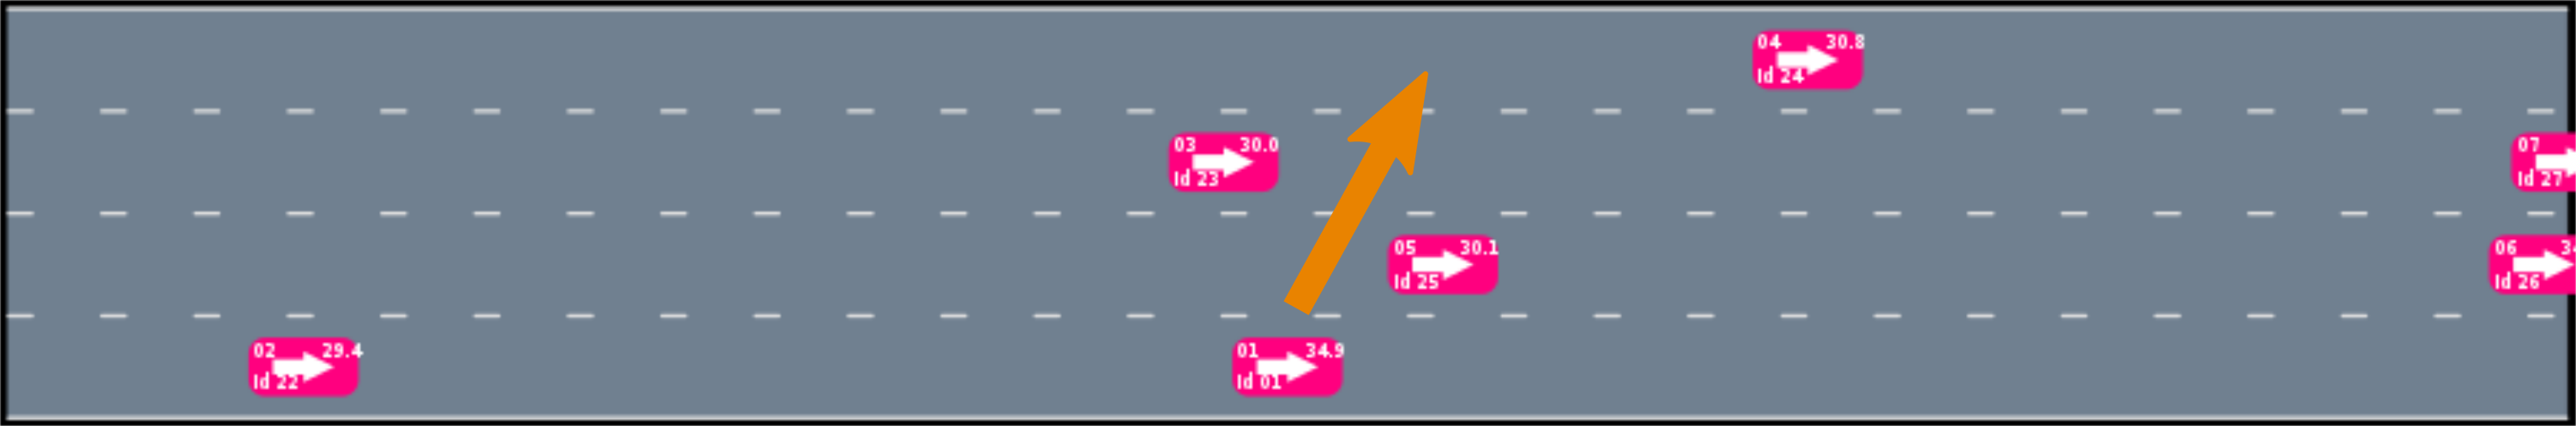
\includegraphics[width=\columnwidth]{media/scene.png}
    \caption[Lane changing scenario]{The example decision making scenario for this chapter. An autonomous vehicle (bottom center) must travel from the rightmost to leftmost lane within a limited distance.}
    \label{fig:scene}
\end{figure}

Throughout this section, $x$ denotes position in the \emph{longitudinal} direction, that is, the direction that the cars move along the road in meters, and $y$ denotes position in the \emph{lateral} direction, that is, the lane the car occupies in lane units.
The problem can be stated as a discrete-time POMDP defined by the tuple $(\sspace, \aspace, \tdist, \reward, \ospace, \odist)$, which consists of

\begin{itemize}
    \item The state space, $\sspace$: A system state, $$s = (q_0, \{(\ith{\phys},\ith{\beh})\}_{i \in 1..N}) \in \sspace\text{,}$$ consists of the physical state of the ego vehicle ($q_0$), and physical state and behavior model for each of the $N$ other cars in the scene.
The physical state, $$\ith{\phys} = (\ith{x},\ith{y},\ith{\dot{x}},\ith{\dot{y}})\text{,}$$ consists of the car's longitudinal and lateral position and velocity. The internal state (behavior model parameters), $\ith{\beh}$, is drawn from a set of behaviors $\Beh$.
    \item The action space, $\aspace$: An action, $u = (\ego{\ddot{x}}, \ego{\ddot{y}}) \in \aspace$, consists of the longitudinal acceleration and lateral velocity of the \av{} vehicle. The action space is discrete and pruned to prevent crashes (see \cref{sec:action}).
    \item The state transition model, $\tdist: \sspace \times \aspace \times \sspace \to \reals$: The value $\tdist(s,u,s')$ is the probability of transitioning to state $s'$ given that action $u$ is taken by the \av{} at state $s$. This function is implicitly defined by a generative model that consists of a state transition function, $F(\cdot)$, and a stochastic noise process (see \cref{sec:dynamics}).
    \item The reward model, $\reward:\sspace \times \aspace \times \sspace \to \reals$: The reward function, defined in \cref{sec:reward}, rewards reaching the left lane within the distance limit and penalizes unsafe actions.
    \item The observation space, $\ospace$: An observation, $o \in \ospace$ consists of the physical states of all of the vehicles, that is $o=\{p_i\}_{i \in 1..N}$. No information about the internal state is directly included in the observation.
    \item The observation model, $Z: S \times O \to \mathbb{R}$: The value $Z(s',o)$ is the probability of receiving observation $o$ when the system transitions to state $s'$. In these experiments, the physical state is assumed to be known exactly, though it is not difficult to relax this assumption. %Hence, $Z(s',o) = \delta_{\phys'}(o)$ where $\delta_{\phys'}$ is a Dirac delta function with the origin at $\phys'$.
\end{itemize}
The remainder of this section elaborates on this model.

\subsection{Driver Modeling} \label{sec:driver}

The driver models for each car have two components: an acceleration model that governs the longitudinal motion and a lane change model that determines the lateral motion.
In this chapter, the acceleration model is the Intelligent Driver Model (IDM) \cite{treiber2000idm}, and the lane change model is the ``Minimizing Overall Braking Induced by Lane change'' (MOBIL) model \cite{kesting2007mobil}.
Both of these models have a small number of parameters that determine the  behavior of the drivers.
The distribution of these parameters in the population of vehicles will be denoted $\Theta$.

% IDM Model Description
\subsubsection{IDM}

The IDM Model was developed as a simple model for ``microscopic'' simulations of traffic flows and is able to reproduce some phenomena observed in real-world traffic flows.
It determines the longitudinal acceleration for a human-driven car, $\ddot{x}$, based on the desired distance gap to the preceding car, $g$, the absolute velocity, $\dot{x}$, and the velocity relative to the preceding car $\Delta \dot{x}$.
The longitudinal acceleration is governed by the following equation:
\begin{equation}
    \ddot{x}_\text{IDM} = a \left[ 1 - \left( \frac{\dot{x}}{\dot{x}_0} \right)^{\delta} - \left(\frac{g^*(\dot{x}, \Delta \dot{x})}{g}\right)^2 \right] \text{,}
\end{equation}
where $g^*$ is the desired gap given by
\begin{equation} \label{eqn:gstar}
    g^*(\dot{x}, \Delta \dot{x}) = g_0 + T \dot{x} + \frac{\dot{x}\Delta \dot{x}}{2 \sqrt{a b}} \text{.}
\end{equation}
Brief descriptions and values for the parameters not defined here are provided later in \cref{tab:modelparams}.

A small amount of noise is also added to the acceleration
\begin{equation}
    \ddot{x} = \ddot{x}_\text{IDM} + w \text{,}
\end{equation}
where $w$ is a random variable with a triangular distribution with support between $-a/2$ and $a/2$. In cases where the noise might cause a hard brake or lead to a state where a crash is unavoidable, the distribution is scaled appropriately.

\subsubsection{MOBIL}

The MOBIL model makes the decision to change lanes based on maximizing the acceleration for the vehicle and its neighbors.
When considering a lane change, MOBIL first ensures that the safety criterion $\tilde{\ddot{x}}_\text{follow} \geq -b_\text{safe}$, where $\ddot{x}_n$ will be the acceleration of the following car if the lane change is made and $b_\text{safe}$ is the safe braking limit. 
It then makes the lane change if the following condition is met
\begin{equation}
    \tilde{\ddot{x}}_c - \ddot{x}_c + p \left( \tilde{\ddot{x}}_n - \ddot{x}_n + \tilde{\ddot{x}}_o - \ddot{x}_o \right) > \Delta a_\text{th}
\end{equation}
where the quantities with tildes are calculated assuming that a lane change is made, the quantities with subscript $c$ are quantities for the car making the lane change decision, those with $n$ are for the new follower, and those with $o$ are for the old follower.
The parameter $p \in [0,1]$ is the politeness factor, which represents how much the driver values allowing other vehicles to increase their acceleration. The parameter $\Delta a_\text{th}$ is the threshold acceleration increase to initiate a lane changing maneuver. Parameter values are listed in \cref{tab:modelparams}.


\subsection{Physical Dynamics} \label{sec:dynamics}

The physical dynamics are simplified for the sake of computational efficiency. Time is divided into discrete steps of length $\dt$.
The longitudinal dynamics assume constant acceleration, and the lateral dynamics assume constant velocity over a time step, that is
\begin{eqnarray*}
    x'&=&x + \dot{x} \dt + \frac{1}{2} \ddot{x} \dt^2 \\
    \dot{x}'&=&\dot{x} + \ddot{x} \dt \\
    y'&=&y + \dot{y} \dt \text{.}
\end{eqnarray*}

There is a physical limit to the braking acceleration, $\bmax$.
Lateral velocity is allowed to change instantly because cars on a freeway can achieve the lateral velocity needed for a lane change in time much shorter than $\dt$ by steering.
If MOBIL determines that a lane change should be made, the lateral velocity, $\dot{y}$, is set to $\dot{y}_\text{lc}$.
Lane changes are not allowed to reverse. Once a lane change has begun, $\dot{y}$ remains constant until the lane change is completed (this is the reason that $\dot{y}$ is part of the state).
When a vehicle passes over the midpoint of a lane, lateral movement is immediately stopped so that lane changes always end at exactly the center of a lane.

Since MOBIL only considers cars in adjacent lanes, there must be a coordination mechanism so that two cars do not converge into the same lane simultaneously.
In order to accomplish this, if two cars begin changing into the same lane simultaneously, and the front vehicle is within $g^*$ of the rear vehicle, the rear vehicle's lane change is canceled.

In order to reduce the computational demands of decision-making, only \SI{50}{\meter} of road in front of the \av{} and \SI{50}{\meter} behind are modeled. %(see \cref{fig:scene}).
Thus, a model for vehicle entry into this section is needed.
If there are fewer than $N_\text{max}$ vehicles on the road, a new vehicle is generated.
First, a behavior for the new vehicle is drawn from $\Theta$, and the initial speed is set to $\dot{x}_0 + \sigma_\text{vel} w_0$, where $\dot{x}_0$ is the desired speed from the behavior model and $w_0$ is a zero-mean, unit-variance, normally distributed random variable that is independent for each car.
If this speed is greater than the \av{}'s speed, the new vehicle will appear at the back of the road section; if it is less, it will appear at the front.
For each lane, $g^*$ is calculated, either for the new vehicle if the appearance is at the back or for the nearest following vehicle if the appearance is at the front.
The new vehicle appears in the lane where the clearance to the nearest car is greatest.
If no clearance is greater than $g^*$, the new vehicle does not appear.

Once the \av{} reaches the target lane ($y = y_\text{target}$) or passes the distance limit ($x \geq L$), the problem terminates.

For convenience, throughout this chapter, the behavior described so far will be denoted compactly by the state transition function
    \begin{equation}
        s' = F(s,u,w) \text{.}
    \end{equation}

\subsection{Action Space for Crash-Free Driving} \label{sec:action}

At each time step, the planner for the \av{} must choose the longitudinal and lateral acceleration.
For simplicity, the vehicle chooses from up to ten discrete actions which are shown in \cref{fig:actions}.
The vehicle may make an incremental decrease or increase in speed or maintain speed, and it may begin a left or right lane change or maintain the current lane.
The combination of these adjustments make up nine of the actions.
The final action is a braking action determined dynamically based on the speed and position of the vehicle ahead.
At each time step, the maximum permitted acceleration, $a_\text{max}$, is the maximum acceleration that the \av{} could take such that, if the  vehicle ahead immediately begins braking at the physical limit, $\bmax$, to a stop, the \av{} will still be able to stop before hitting it without exceeding physical braking limits itself.
The braking action is $(\ego{\ddot{x}}, \ego{\ddot{y}}) = (\min \{a_\text{max}, -b_\text{nominal} \}, 0)$.

\begin{figure}[tb]
    \centering
    \includestandalone[mode=buildnew,width=0.5\textwidth]{action_space}
    
    \caption{Lane changing action space}
    \label{fig:actions}
\end{figure}


The inclusion of the dynamic braking action guarantees that there will always be an action available to the \av{} to avoid a crash.
At each step, the action space is pruned so that if $\ego{\ddot{x}} > a_\text{max}$ or if a lane change leads to a crash, that action is not considered.
Since the IDM and MOBIL models are both crash-free \cite{kesting2009agents}, and actions that lead to crashes for the \av{} are not considered, no crashes occur in the simulation.
Eliminating crashes in our model is justifiable because it is likely that in an actual autonomous vehicle a high-level planning system would be augmented with a low-level crash prevention system to increase safety and facilitate certification. 
In addition, it is difficult to model driver behavior in the extraordinary case of a crash. 

\subsection{Reward Function and Objectives} \label{sec:reward}

The qualitative objectives in solving this problem are to reach the target lane within a specified distance, $L$, and maintain the comfort and safety of both the \av{} and the other nearby vehicles.
Thus, the following two metrics will be used to evaluate planning performance: 1) the fraction of episodes in which the \av{} reaches the target lane, and 2) the fraction of episodes in which \emph{any} vehicle operates in an unsafe manner.
For this work, hard braking and unusually slow velocity are considered unsafe.
A hard braking maneuver is defined as $\ddot{x} < -b_\text{hard}$ and slow velocity as $\dot{x} < \dot{x}_\text{slow}$, where $b_\text{hard}$ and $\dot{x}_\text{slow}$ are chosen to be uncomfortably abrupt deceleration or slow travel that might result in an accident in real conditions (see \cref{tab:params}).
In addition to quantifying safety, hard braking also serves as a proxy for comfort.

In order to encourage the planner to choose actions that will maximize these metrics, the reward function for the POMDP is defined as follows: 
\begin{equation} \label{eqn:reward}
    % R(s, s') = \mathbf{1}(\ego{y}=y_\text{target}) - \lambda \sum_{i=1}^N \mathbf{1}(\ith{\dot{x}}'- \ith{\dot{x}} < -b_\text{hard} \Delta t) \text{.}
    \reward(s, a, s') = \text{in\_goal}(s') - \lambda \left(\text{any\_hard\_brakes}(s, s') + \text{any\_too\_slow}(s')\right)
\end{equation}
where
\begin{align}
    \text{in\_goal}(s') &= \mathbf{1}(\ego{y} = y_\text{target}, \ego{x} \leq L) \text{,}\\
    \text{any\_hard\_brakes}(s,s') &= \max_{i \in 1..N}\{\mathbf{1}(\ith{\dot{x}}' - \ith{\dot{x}} < -b_\text{hard} \Delta t) \} \text{,}\\
    \text{any\_too\_slow}(s') &= \max_{i \in 1..N} \{\mathbf{1}(\ith{\dot{x}} < \dot{x}_\text{slow})\} \text{.}
\end{align}
That is, there is a positive reward for reaching the target lane within the distance limit, and hard brakes and slow velocity for any car are penalized.
The weight $\lambda$ balances the competing goals and can be adjusted to create an approximate curve of Pareto-optimal solutions.

\subsection{Initial Scenes} \label{sec:initial}

Initial scenes for the simulations are generated by beginning a simulation with only the \av{} on the road section and then simulating 200 steps to allow other vehicles to accumulate in the scene.

\section{Solution Approaches}

Each of the solution techniques is based on MCTS-DPW (\cref{sec:mcts,sec:uct,sec:dpw}), but handles uncertainty in the internal states differently.

\subsection{Approach 1: Assume normal behavior}

The first performance baseline is established by planning as if all cars behave according to a single static ``normal'' internal state (see \cref{tab:modelparams}).
In this case, the problem is an MDP, which is solved using the MCTS-DPW algorithm.
This is an overconfident baseline --- it plans assuming it knows more about the other drivers than is justified by the information it has collected.

\subsection{Approach 2: Model all uncertainty as outcome uncertainty (Naive MDP)}

The second performance baseline is established by planning as if all uncertainty is simply outcome uncertainty, that is, as if the problem were an MDP with a state consisting only of the physical state and the internal states random variables, independent at each timestep, distributed according to the internal state distribution $\Theta$. 
This model would be the result of fitting a Markov model with only the physical state based on data from all drivers.
The MDP is again solved using the MCTS-DPW algorithm.

\subsection{Approach 3: Mean Model Predictive Control} \label{sec:mpc}

Since information about the human's internal state can be inferred by observing the car's physical motion, performance superior to either of the baselines can be achieved by estimating $\beh$ online.
This is accomplished with a particle filter (see \cref{sec:particle}, \cite{thrun2005probabilistic}).
Filtering is independent for each car, but all of the behavior parameters for a given car are estimated jointly.
There are two versions of the filter.
In the first version, a particle, $\hat{\theta}$, consists of values of all model parameters.
In the second version, all parameters are assumed perfectly correlated (see \cref{sec:dist}), so a particle consists of only a single value, the ``aggressiveness''.

The belief at a given time consists of the exactly known physical state, \phys, and a collection of $M$ particles, $\{\hat{\theta}^k\}_{k=1}^M$, along with associated weights, $\{W^k\}_{k=1}^M$.
To update the belief when action $u$ is taken, $M$ new particles are sampled with probability proportional to the weights, and sampled noise values $\{\hat{w}^k\}_{k=1}^M$ are used to generate new states according to ${\hat{s}^k}{'} = F((\phys, \hat{\theta}^k), u, \hat{w}^k)$.
The new weights are determined by approximating the conditional probability of the particle given the observation:
% \begin{equation*}
% {W^k}{'} = \left.
% \begin{cases}
% \exp\left(- \frac{(\dot{x}'-\hat{\dot{x}}')^2}{2 \sigma_\text{vel}^2} \right) & \text{if } y' = \hat{y}' \\
% \gamma_\text{lane} \exp\left(- \frac{(\dot{x}'-\hat{\dot{x}}')^2}{2 \sigma_\text{vel}^2} \right) & \text{o.w.}
% \end{cases} \right\} \appropto \operatorname{Pr}\left(\left.\hat{\theta}^k \right| o \right)
% \end{equation*}
\begin{equation*}
{W^k}{'} = \left.
\begin{cases}
    \max\left\{0, \frac{a - 2 \, \left| \dot{x}' - \hat{\dot{x}}' \right|}{a} \right\} & \text{if } y' = \hat{y}' \\
\gamma_\text{lane} \max\left\{0, \frac{a - 2 \, \left| \dot{x}' - \hat{\dot{x}}' \right|}{a} \right\} & \text{o.w.}
\end{cases} \right\} \appropto \operatorname{Pr}\left(\left.\hat{\theta}^k \right| o \right)
\end{equation*}
where $\dot{x}'$ and $y'$ are taken from the observation, $\hat{\dot{x}}'$ and $\hat{\dot{y}}'$ are from ${\hat{s}^k}{'}$, the max expression is proportional to the probability density of the acceleration noise triangular distribution (ignoring the effects of the collision mitigation modifications), and $\gamma_\text{lane} \in [0,1]$ is a hand-tuned parameter that penalizes incorrect lane changes (see \cref{tab:params}).

% the below paragraph is not true anymore
% In order to prevent particle deprivation, during the resampling step, Gaussian noise with standard deviation proportional to the sample standard deviation of the current particle set is added to \SI{10}{\percent} of the new samples.

Model predictive control (MPC) is a widely used family of control techniques that use an imperfect model and feedback measurements to choose actions \cite{garcia1989model}. At each time step, a model predictive controller calculates a sequence of control actions that will maximize a reward function of the states visited up to a future horizon given that the system behaves according to a model. The first control action in this optimized sequence is executed, and the process is repeated after a new measurement is received.

In the mean model predictive control (MMPC) approach, this particle filter is used to estimate the internal state for each driver. At each step, MPC uses the MDP that results from assuming that each driver has the internal state corresponding to the mean of the particles in the belief approximation as the model for planning. Each time a new observation is received, the particle filter is updated and MCTS-DPW determines the best action for the resulting MDP.

\subsection{Approach 4: QMDP}

The fourth approach uses MCTS-DPW to solve the QMDP approximation of the POMDP (see \cref{sec:qmdp}).

\subsection{Approach 5: POMCPOW}

The final approach uses the POMCPOW solver described in \cref{sec:pomcpow}.
Though there is no theoretical guarantee that this approach will converge to an optimality, this is the closest approximation to the exact POMDP solution

\section{Results}

The computational results from this study are designed to meet the two goals of 1) quantifying the size of the gap between the baseline control algorithm and the maximum potential lane change performance and 2) showing which cases internal state estimation and POMDP planning can approach the upper bound on performance.
Experiments are carried out in three scenarios, each with a different distribution of internal states.
In each of these scenarios, each of the approaches described in \cref{sec:solution} are compared with an approximate upper performance bound obtained by planning with perfect knowledge of the behavior models.

\subsection{Driver Model Distribution Scenarios} \label{sec:dist}

For the numerical testing, three internal state distribution scenarios were considered.
In all of these scenarios, drivers behave according to the IDM and MOBIL models presented in \cref{sec:driver}, however the IDM and MOBIL parameter values are distributed differently.

\Cref{tab:modelparams} shows typical parameter values for aggressive, timid, and normal drivers.
The values are taken from \citet{kesting2009agents}, but some have been adjusted slightly so that the parameters for the normal driver are exactly half way between values for the timid and aggressive drivers.
In all three of the scenarios, the \emph{marginal} distributions of the parameters are uniformly distributed between the aggressive and timid values.
The difference between the scenarios is the correlation of the parameter values.
In Scenario 1, all of the parameters are independently distributed.
In Scenario 2, all of the parameters are perfectly correlated so that all parameters are deterministic functions of the aggressiveness of the driver.
Scenario 3 uses a distribution between these two extremes.
In this scenario, values are drawn from a Gaussian copula with covariance matrix
\begin{equation}
    \Sigma = \begin{bmatrix}
        1 & \dots & \rho \\
        \vdots & \ddots & \vdots \\
        \rho & \dots & 1
    \end{bmatrix}\text{,}
\end{equation}
that is, a matrix with 1 along the diagonal and $\rho$ elsewhere.
The values are then scaled and translated to lie between the aggressive and normal limits.
For Scenario 3, the value of $\rho$ is \num{0.75}, and Scenarios 1 and 2 can be thought of as limiting cases where $\rho$ approaches 0 and 1, respectively.
In Scenario 1, the first version of the particle filter, which estimates all of the model parameters jointly, is used, whereas in Scenarios 2 and 3, the second version of the particle filter that assumes fully correlated parameters is used, that is, it only estimates a single ``aggressiveness'' parameter for each car.
The small scatter plots in \cref{fig:gaps,fig:075} illustrate the level of correlation by plotting sampled values of two of the parameters.

\begin{table}[tbph]
    \caption{IDM and MOBIL parameters for different driver types.}
    \centering
    \footnotesize
    \begin{tabular}{@{}llrrr@{}}
        \toprule
        IDM Parameter & & \hspace{-3ex} Timid & Normal & Aggressive \\
        \midrule
        Desired speed (\si{\meter\per\second}) & $\dot{x}_0$ & 27.8 & 33.3 & 38.9 \\
        Desired time gap (\si{\second}) & $T$ & 2.0  & 1.5 & 1.0 \\
        Jam distance (\si{\meter})     & $g_0$ & 4.0  & 2.0 & 0.0 \\
        Max acceleration (\si{\meter\per\second\squared}) & $a$ & 0.8  & 1.4 & 2.0 \\
        Desired deceleration (\si{\meter\per\second\squared}) & $b$ & 1.0  & 2.0 & 3.0 \\
        \midrule
        MOBIL Parameter & & \hspace{-3ex} Timid & Normal & Aggressive \\
        \midrule
        Politeness & $p$ & 1.0 & 0.5 & 0.0 \\
        Safe braking (\si{\meter\per\second\squared}) & $b_\text{safe}$ & 1.0 & 2.0 & 3.0 \\
        Acceleration threshold (\si{\meter\per\second\squared}) & $a_\text{thr}$ & 0.2 & 0.1 & 0.0 \\
        \bottomrule
    \end{tabular}
    \label{tab:modelparams}
\end{table}

\begin{table}[tbph]
    \caption{Various simulation parameters}
    \center
    \begin{tabular}{@{}llr@{}}
        \toprule
            Parameter & Symbol & Value \\
        \midrule
            Simulation time step & $\Delta t$ & \SI{0.75}{\second} \\
            Max vehicles on road & $N_\text{max}$ & \num{10} \\
            Lane change rate & $\dot{y}_\text{lc}$ & \SI{0.67}{lanes\per\second} \\
            Distance limit & $L$ & \SI{1000}{\meter} \\
            Velocity noise standard deviation & $\sigma_\text{vel}$ & \SI{0.5}{\meter\per\second} \\
            Physical braking limit & $b_\text{max}$ & \SI{8.0}{\meter\per\second\squared} \\
            Penalized hard braking limit & $b_\text{hard}$ & \SI{4.0}{\meter\per\second\squared} \\
            Penalized minimum speed & $\dot{x}_\text{slow}$ & \SI{15}{\meter\per\second} \\
            UCT exploration parameter & $c$ & 8 \\
            DPW linear parameter & $k$ & 4.5 \\
            DPW exponent parameter & $\alpha$ & 0.1 \\
            MCTS search depth & & 40 \\
            MCTS iterations per step & & 1000 \\
            Particle filter wrong lane factor & $\gamma_\text{lane}$ & 0.05 \\
            Number of Particles (Joint Parameter Filter) & $M$ & 5000 \\
            Number of Particles (Aggressiveness Filter) & $M$ & 2000 \\
            Reward ratios for points on approximate Pareto curves & $\lambda$ & 0.5, 1, 2, 4, 8 \\
        \bottomrule
    \end{tabular}
    \label{tab:params}
\end{table}

\subsection{Performance Results}

\begin{figure}[p]
    \centering
    \begin{subfigure}{\textwidth}
        \centering
        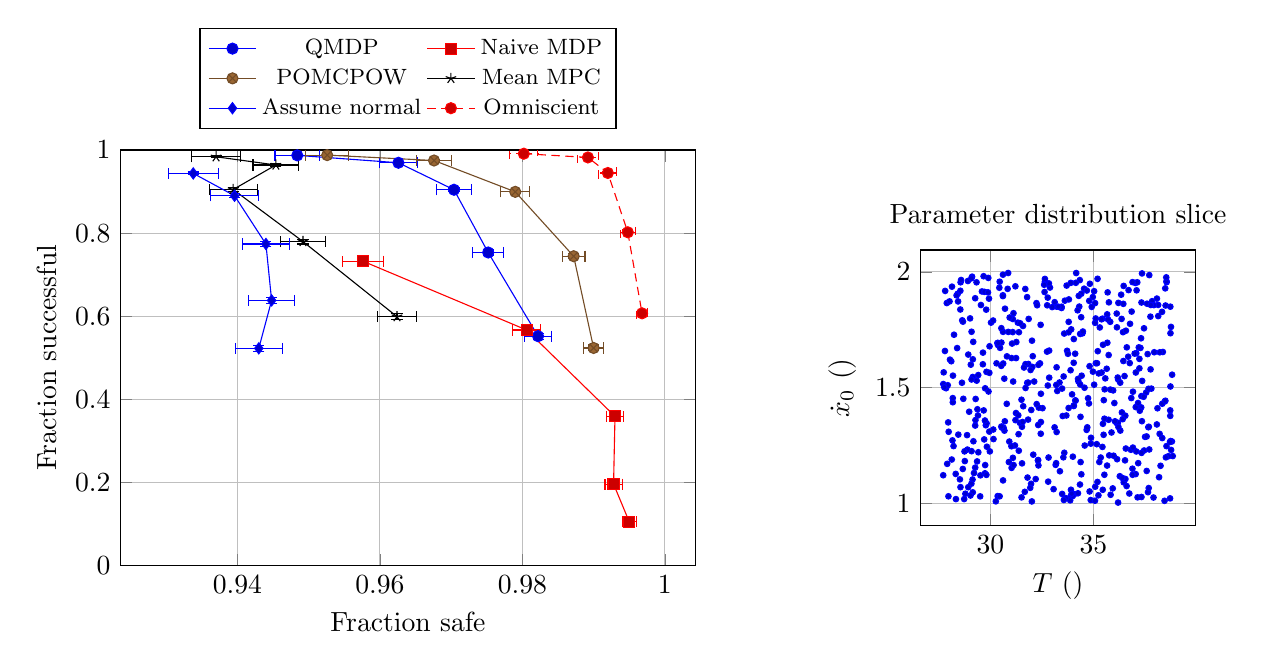
\begin{tikzpicture}[]
\begin{axis}[height = {2.7in}, ylabel = {Fraction successful}, ymax = {1.0}, xlabel = {Fraction safe}, legend style={at={(0.5,1.05), font=\footnotesize}, anchor=south, font=\footnotesize}, legend columns=2, grid=both, ymin = {0.0}, width = {3.5in}]\addplot+ [
, error bars/.cd, 
x dir=both, x explicit, y dir=both, y explicit]
table [
x error plus=ex+, x error minus=ex-, y error plus=ey+, y error minus=ey-
] {
x y ex+ ex- ey+ ey-
0.9484 0.9872 0.003128809020886042 0.003128809020886042 0.0015898860171438421 0.0015898860171438421
0.9626 0.9694 0.0026835961577084603 0.0026835961577084603 0.002435962804099576 0.002435962804099576
0.9704 0.9044 0.0023970642843771945 0.0023970642843771945 0.004158796354406325 0.004158796354406325
0.9752 0.7534 0.002199536222006431 0.002199536222006431 0.006096320285566137 0.006096320285566137
0.9822 0.552 0.0018701153617606734 0.0018701153617606734 0.007033426890127155 0.007033426890127155
};
\addlegendentry{QMDP}
\addplot+ [
, error bars/.cd, 
x dir=both, x explicit, y dir=both, y explicit]
table [
x error plus=ex+, x error minus=ex-, y error plus=ey+, y error minus=ey-
] {
x y ex+ ex- ey+ ey-
0.9576 0.7326 0.002849924984009729 0.002849924984009729 0.00625997487671408 0.00625997487671408
0.9806 0.5668 0.001950766284776213 0.001950766284776213 0.007008378947737845 0.007008378947737845
0.993 0.359 0.0011791853525290762 0.0011791853525290762 0.006784762825723593 0.006784762825723593
0.9928 0.196 0.0011957917810374468 0.0011957917810374468 0.005614544026091883 0.005614544026091883
0.995 0.1054 0.0009975966318146623 0.0009975966318146623 0.004343033546736354 0.004343033546736354
};
\addlegendentry{Naive MDP}
\addplot+ [
, error bars/.cd, 
x dir=both, x explicit, y dir=both, y explicit]
table [
x error plus=ex+, x error minus=ex-, y error plus=ey+, y error minus=ey-
] {
x y ex+ ex- ey+ ey-
0.9526 0.9878 0.003005404214227774 0.003005404214227774 0.0015526474625067136 0.0015526474625067136
0.9676 0.9748 0.0025042568279735533 0.0025042568279735533 0.0022167486990994295 0.0022167486990994295
0.979 0.8994 0.0020279601880966334 0.0020279601880966334 0.00425435634492246 0.00425435634492246
0.9872 0.7444 0.0015898860171438376 0.0015898860171438376 0.006169387349490527 0.006169387349490527
0.99 0.5236 0.0014072654615302116 0.0014072654615302116 0.007063893240808725 0.007063893240808725
};
\addlegendentry{POMCPOW}
\addplot+ [
, error bars/.cd, 
x dir=both, x explicit, y dir=both, y explicit]
table [
x error plus=ex+, x error minus=ex-, y error plus=ey+, y error minus=ey-
] {
x y ex+ ex- ey+ ey-
0.937 0.9838 0.0034363587869054783 0.0034363587869054783 0.001785539030636411 0.001785539030636411
0.9454 0.964 0.0032133834453163725 0.0032133834453163725 0.002634803301517503 0.002634803301517503
0.9394 0.905 0.0033745822794995326 0.0033745822794995326 0.004147100154076068 0.004147100154076068
0.9492 0.7798 0.0031057690126975205 0.0031057690126975205 0.005860824332154153 0.005860824332154153
0.9624 0.599 0.0026904824361344134 0.0026904824361344134 0.006931768164182681 0.006931768164182681
};
\addlegendentry{Mean MPC}
\addplot+ [
, error bars/.cd, 
x dir=both, x explicit, y dir=both, y explicit]
table [
x error plus=ex+, x error minus=ex-, y error plus=ey+, y error minus=ey-
] {
x y ex+ ex- ey+ ey-
0.9338 0.9438 0.0035165302781348935 0.0035165302781348935 0.0032573661272287694 0.0032573661272287694
0.9396 0.89 0.003369367674758206 0.003369367674758206 0.00442537193729029 0.00442537193729029
0.944 0.7738 0.00325190943646908 0.00325190943646908 0.0059172387769084464 0.0059172387769084464
0.9448 0.638 0.003229965717419773 0.003229965717419773 0.006797090560527933 0.006797090560527933
0.943 0.5228 0.0032790776858888245 0.0032790776858888245 0.007064418815630945 0.007064418815630945
};
\addlegendentry{Assume normal}
\addplot+ [
, error bars/.cd, 
x dir=both, x explicit, y dir=both, y explicit]
table [
x error plus=ex+, x error minus=ex-, y error plus=ey+, y error minus=ey-
] {
x y ex+ ex- ey+ ey-
0.9802 0.9912 0.001970372673809381 0.001970372673809381 0.0013209318575136467 0.0013209318575136467
0.9892 0.9822 0.0014618821497931905 0.0014618821497931905 0.0018701153617606734 0.0018701153617606734
0.992 0.9448 0.0012599672628686462 0.0012599672628686462 0.0032299657174197694 0.0032299657174197694
0.9948 0.802 0.001017250686798468 0.001017250686798468 0.00563609378121247 0.00563609378121247
0.9968 0.607 0.0007987988582385328 0.0007987988582385328 0.006907947882605195 0.006907947882605195
};
\addlegendentry{Omniscient}
\end{axis}
\begin{axis}[height = {2in}, ylabel = {$\dot{x}_0$ (\si{\meter\per\second})}, title = {Parameter distribution slice}, xlabel = {$T$ (\si{\second})}, xshift=4in, yshift=0.2in, grid=both, width = {2in}]\addplot+[draw=none, mark size = {1}] coordinates {
(34.79690241123805, 1.8746973944071812)
(32.33088698822359, 1.1636077754332113)
(38.46234940897947, 1.4400139243610581)
(33.89999414484549, 1.0306215457264516)
(32.629648497566386, 1.9130838428140544)
(35.67548520152797, 1.6938090009854834)
(38.14414045085168, 1.8090483607343504)
(28.92661870133864, 1.6427009048346797)
(35.54390697121511, 1.492586609113691)
(37.84840296204164, 1.873532548458079)
(35.287091081628596, 1.1784221692038184)
(34.67117668877091, 1.3171631273245603)
(37.55882632525877, 1.4786228237903052)
(31.19173003199198, 1.2499753840224004)
(28.4178286366807, 1.905510128373736)
(36.466279255619455, 1.9393272282304284)
(29.796628881672316, 1.836882006675407)
(28.786232407392937, 1.0413031156475263)
(37.648376778028336, 1.0478942069493047)
(34.0476407621513, 1.7097107377171146)
(31.787751331806874, 1.5204234771116094)
(33.50840898632556, 1.3770820442367266)
(35.45369703859319, 1.0582527092116294)
(34.814624625152206, 1.0510721971152106)
(33.69924378712916, 1.940892116044016)
(31.367973225592902, 1.2986714307812355)
(35.1173328713055, 1.6053312673081166)
(36.3446250003244, 1.9014960723259093)
(32.75747979274516, 1.8556620149665404)
(30.70169896224632, 1.3543264302358808)
(37.35828982946927, 1.9934679561089816)
(33.16806235222252, 1.1661313494371794)
(34.78316374096517, 1.431350702450156)
(28.909411110754792, 1.960706678163213)
(29.149232997333, 1.6223319974695511)
(38.34051826829441, 1.2818474734640641)
(29.14337241070168, 1.545813041948128)
(36.1308352182244, 1.8199811891351962)
(38.1074394648648, 1.4106266007835326)
(37.08012839324377, 1.6485844756085457)
(36.279577188686886, 1.1170083755579134)
(31.532258343745657, 1.3305943878088242)
(36.6193447540874, 1.67390890811335)
(28.44372501162216, 1.2967235114378237)
(31.693921268963265, 1.9262883990946138)
(33.799341783480386, 1.7840595054928248)
(31.80238274662397, 1.1110946023483186)
(28.6213518233413, 1.5208521032355908)
(28.183571794480986, 1.5516371659902142)
(30.559542967875426, 1.326767928135903)
(38.80775703921492, 1.2670862909544582)
(38.33882961679038, 1.4302344461884753)
(28.32842116940828, 1.0179600287594135)
(29.810774190761634, 1.5679848637954918)
(35.95727005062043, 1.4877667445412521)
(36.19698483655556, 1.0030752990608187)
(35.73876347824327, 1.3608707670615325)
(37.353001005179756, 1.354727281788758)
(29.28449343907644, 1.450867489143519)
(34.355856519376566, 1.731913845704761)
(37.03089180263208, 1.9523609797854857)
(38.552874097913, 1.9555668262567063)
(34.06859768256475, 1.039241964137901)
(34.414340171985145, 1.1252215571514914)
(29.26236530359105, 1.8861604426456995)
(31.832829329999655, 1.5215209682991049)
(29.74705929749524, 1.1650804401518073)
(38.491834348448926, 1.4432093986725945)
(36.893487599172076, 1.1494777780717231)
(29.16650309612929, 1.697620251739014)
(33.910251168492415, 1.058430310029541)
(31.090322415165737, 1.7963679351579314)
(31.858290560263267, 1.796878158946281)
(29.41503023166148, 1.2204196876620552)
(35.57583083140365, 1.5397929007002116)
(38.74825869538596, 1.2689796974791383)
(34.70164328050001, 1.3283171452915643)
(31.37807948321803, 1.2271756098900413)
(38.45097570742132, 1.0105968662763483)
(30.139997015089005, 1.3187913336928037)
(29.739086861790206, 1.1295360164707589)
(32.78776683355239, 1.5089449027569686)
(36.837610078191965, 1.4547571855942525)
(29.112925152418498, 1.97936026833434)
(29.04999909329045, 1.5990061671327507)
(27.80599182929105, 1.9178049909217068)
(35.813584053816484, 1.7843349514951152)
(30.804402965301115, 1.6349688845996007)
(29.08628597025123, 1.5350645311430546)
(30.614371172558357, 1.0988313184554104)
(36.20192611498645, 1.534896722165889)
(35.39631803910467, 1.5649911261913774)
(28.177036551811845, 1.4366271690607197)
(37.32657468831977, 1.4632175574001454)
(37.506742359690975, 1.286959794556308)
(32.44407291263385, 1.300584053659912)
(35.17591839734406, 1.6053655673362146)
(32.851732552002915, 1.6598138968317013)
(28.548592428772753, 1.06966732701888)
(38.36935273376649, 1.6538973550307743)
(29.355654263176508, 1.1808159271861665)
(36.148499281173024, 1.1904795560246018)
(34.12096140751532, 1.4445275798703239)
(35.0811280665884, 1.779817742433471)
(35.49358158573741, 1.295951482158264)
(31.43415336969513, 1.3474987826222677)
(36.53349523705934, 1.1854781281686053)
(37.6027800468338, 1.8625153501102418)
(30.43431007259245, 1.931635246122652)
(29.327396429959226, 1.9550066968589908)
(32.40676135303459, 1.6047869851630672)
(30.61101658295737, 1.9880718203375443)
(38.769975550200286, 1.230472989804727)
(29.504415207408318, 1.029876670043506)
(31.213857926029945, 1.9377188462247374)
(37.051197816559345, 1.126147147426688)
(36.686608371886784, 1.6335421169248112)
(34.270277545629654, 1.527290873804888)
(29.134542355975462, 1.1026570361688843)
(29.8063692388397, 1.1227294145662376)
(34.04325143824957, 1.6071613353170962)
(36.43588791293467, 1.739540298034852)
(38.07840270537357, 1.3407076602475196)
(38.50203093606017, 1.8547388081895688)
(30.031613404815012, 1.7808522308727246)
(30.60672163727217, 1.8989103657502986)
(37.077723995925474, 1.2238743179348948)
(31.67028570368791, 1.049437916617303)
(31.05222897794565, 1.690223246209014)
(27.851315745419274, 1.4973724938031538)
(38.330884294039855, 1.8274102417674107)
(32.197896042704485, 1.104705952606801)
(36.99935528722166, 1.6468619081826747)
(34.114006480548774, 1.64636954111271)
(34.917977625023326, 1.8487696719733437)
(33.79708164313204, 1.4117333758158472)
(35.44390883136532, 1.79801812368519)
(32.23688675966768, 1.8650422950180132)
(38.818639201747715, 1.5556835329854404)
(30.621298225901405, 1.6040838855419075)
(28.76003875878276, 1.182268689936856)
(33.21260171749708, 1.5875773188124296)
(36.82026317832538, 1.2310510975082343)
(27.96586929820616, 1.030113237907791)
(33.373841058304805, 1.1384566423881899)
(35.25805393067896, 1.5612076858961235)
(31.243284635569335, 1.3899327914329178)
(34.162882802425514, 1.9950190213093804)
(32.74798663968328, 1.6553287044532972)
(33.614017558551076, 1.8756968482887584)
(31.018696385612746, 1.2464700709947358)
(36.14126049418779, 1.7604681445223822)
(35.08113802591705, 1.8651195933314513)
(33.477775702658406, 1.4956908235191766)
(36.12189152216062, 1.3470766488077006)
(29.780296287955057, 1.3372615067561926)
(32.12503876879171, 1.5261396270532426)
(35.68941389523972, 1.9114952502427967)
(36.91559505405698, 1.2406804856198552)
(34.739943164634475, 1.4540044742734426)
(37.58456938113252, 1.1396440789620752)
(34.4116404438892, 1.905691309823502)
(33.87224232117965, 1.012617672277038)
(37.66332388637268, 1.3287017352706862)
(29.932420682228166, 1.8845112381578442)
(34.00169346598638, 1.2014157288930343)
(29.145066244703738, 1.047295903410718)
(30.1516202107506, 1.2774433904566356)
(32.316503624588265, 1.186905985388637)
(30.45119283915048, 1.9576529641044194)
(27.884384648441944, 1.8653387195264814)
(36.30493201570267, 1.314015696021556)
(34.42968012121763, 1.5513727562826976)
(36.54898733305876, 1.3783810718512233)
(29.087078212877667, 1.2251467645343672)
(34.04795028683671, 1.42036866729439)
(32.89122759602115, 1.932367840647952)
(38.84985409037526, 1.2041075380500967)
(29.262887460998016, 1.3358882008989137)
(34.81277081891696, 1.592477918200708)
(31.98364724775052, 1.4032539290955293)
(31.84158991091455, 1.601916262002125)
(36.453008355517035, 1.6148394646068434)
(35.76682370904995, 1.2070528140469898)
(36.575533068749365, 1.7458167641501119)
(29.078504012840842, 1.0847287477091059)
(30.681802275421447, 1.3139823479376933)
(33.68769243224376, 1.3794968696438135)
(28.543645954992474, 1.9184454824087112)
(32.84043089970852, 1.9503742811060913)
(32.64584691587665, 1.9577013861400179)
(30.613891293466786, 1.7409140921199213)
(28.634844291038615, 1.7906939046871146)
(31.085298612249826, 1.7398109907987571)
(31.53618981631512, 1.17249145289402)
(30.536340578730723, 1.6944830311272003)
(30.64180597757236, 1.3260609020105594)
(33.11959231943374, 1.869078357066173)
(34.37701128810902, 1.1780497419968725)
(28.10267236118751, 1.6138871530646794)
(34.97588068674558, 1.5689160542950207)
(37.43817354795076, 1.4602865621186403)
(28.55479280577856, 1.9551532047228843)
(35.97829621403939, 1.2055909780634069)
(34.56773669885426, 1.4994778767809556)
(30.60711581816141, 1.895365221803583)
(31.58249323160836, 1.7662876269063104)
(34.97092288776974, 1.8914892701239947)
(30.527992327766633, 1.5938714215683765)
(27.951678164654982, 1.3495893799618355)
(28.017718090299496, 1.8725093635170103)
(38.71701437369716, 1.2652462168671728)
(36.46856651977355, 1.0905942827708408)
(37.31866256511398, 1.4143655110523008)
(29.949450585049142, 1.5638073649100326)
(36.4200886620777, 1.3635558018125278)
(32.03762461957875, 1.5893147665574303)
(36.76223085968457, 1.6058623413173108)
(33.999940320897174, 1.0315203067065124)
(34.873314257173455, 1.2577262557175055)
(35.465752039223545, 1.6850585613410947)
(35.834775380607624, 1.036738567575581)
(36.70530845775399, 1.9212975903439689)
(36.17964970367275, 1.5435135081799745)
(38.48518875826713, 1.9288642636628794)
(29.95889750687044, 1.6785522567532658)
(32.45081089013532, 1.351203346709172)
(29.589995865225493, 1.9155065003072855)
(32.33266883382916, 1.5982963024152372)
(31.030088892283487, 1.1529111131317102)
(29.333989798418507, 1.530044081222619)
(32.52979709721962, 1.4110319436450809)
(29.74642922029044, 1.4969195443908458)
(37.62986117892169, 1.6447958656875359)
(37.95039532517879, 1.6527728724394053)
(35.39267930529486, 1.795166980026828)
(28.432689206622868, 1.872398074168308)
(28.541247375497093, 1.8375259137941788)
(36.367279537585404, 1.7968663797820208)
(27.90394360469155, 1.170334916678653)
(31.24620466699098, 1.6275037158646977)
(37.33118848189446, 1.8677385581699797)
(34.868923748849646, 1.013921132651612)
(33.45326507001973, 1.8440056688529682)
(34.57793277587389, 1.2495602131582078)
(29.515627238721002, 1.1206551983158337)
(32.34943001085545, 1.4132015742538637)
(35.08765672434117, 1.0715199641788222)
(28.885210120350127, 1.2320432632501352)
(28.159384122154147, 1.2717965566526097)
(37.128332083816716, 1.9551072157229679)
(32.31978669763658, 1.3382333261992203)
(35.19999069877123, 1.9702256444596404)
(30.935173842547048, 1.802871704999311)
(28.17556778001731, 1.4545378181717274)
(31.702889432123257, 1.6012845973176555)
(29.639593034171963, 1.6511155840944438)
(35.82046190470108, 1.491353859048626)
(32.26808825091066, 1.855837489983624)
(32.82297375238989, 1.1977084808448184)
(33.58676974179278, 1.2182683178781886)
(27.795254776959798, 1.6582578429598367)
(30.675010341194856, 1.538550626619082)
(34.46772325438714, 1.7344363506047027)
(36.5532016327695, 1.1048778936367118)
(35.50317864825459, 1.445596060377532)
(35.46105699631721, 1.3433821100293533)
(28.578013124468885, 1.964982813426033)
(32.308547349950786, 1.1849207677214426)
(38.256777985227956, 1.1619984277588402)
(30.861965743875697, 1.995239741571718)
(37.764848902881596, 1.8066851545414648)
(36.90022560226953, 1.1231511010012714)
(32.01935291752141, 1.7026943118909155)
(33.553547513097485, 1.5479979788402978)
(32.01232597220363, 1.0079525417574493)
(33.35497652280619, 1.5221419692480136)
(32.64611341939599, 1.9697070713654719)
(36.5095668049484, 1.5497259893169775)
(29.176356838485166, 1.2679584521191776)
(30.131548315743252, 1.7898537765662255)
(34.34778136577471, 1.08100412914621)
(33.4520436266409, 1.8493751378795773)
(36.18726651688699, 1.3477400659165286)
(37.095308127638326, 1.920463304085399)
(29.71196079990374, 1.9137949791516407)
(32.85433932311724, 1.5428831247355623)
(30.298687356187074, 1.604822435510378)
(34.04392433127704, 1.422781376490324)
(34.372271985306796, 1.3736218153896398)
(32.45112569156182, 1.473356867296689)
(31.564732631519938, 1.3512425287069432)
(31.70758754957295, 1.4983253890304329)
(35.19622678137824, 1.092157384329138)
(38.1411014816305, 1.8573152470632113)
(34.35787500214013, 1.5133583006359113)
(34.25006179280257, 1.0432694661705781)
(30.33941439300583, 1.6926491560115278)
(29.817922791271045, 1.3453562754445105)
(29.079592543249284, 1.972408795203795)
(34.4885569922262, 1.7422680100527166)
(31.385328154799918, 1.7393940421904348)
(29.014922892986565, 1.7991251029075312)
(36.016261273320126, 1.433147355253712)
(33.21186779296181, 1.849880120149472)
(37.71009711350416, 1.986194329382347)
(31.975635385470923, 1.08424308534306)
(33.190633456917965, 1.1733428615427697)
(30.35290247261203, 1.0310082976308688)
(35.73874978291539, 1.640666432894814)
(31.59378777790704, 1.4193736091091458)
(36.91768482540908, 1.4821964029461843)
(27.734837928203874, 1.56585813367934)
(30.917979497089124, 1.2666909224378693)
(38.72598508015691, 1.4016002947542974)
(36.854097158649616, 1.8285440123296364)
(38.63939085936499, 1.2034310506749044)
(31.51178967372038, 1.0254921130015526)
(33.920418674551065, 1.7517781257412357)
(36.04615237714776, 1.3543498602128974)
(30.794744711576165, 1.4298005021747873)
(31.260084253060803, 1.696830643055398)
(34.33998926439865, 1.9646420088233938)
(33.72257959153388, 1.6589657522346624)
(37.81135434833773, 1.4955583380352766)
(29.541539704364677, 1.856851063065449)
(30.531219927867504, 1.3316280050833336)
(37.1426708646404, 1.0255913396836587)
(28.869403264039505, 1.2945201918020455)
(31.091066534585377, 1.1963799838194562)
(31.216694868882975, 1.359283715438054)
(30.449362492835842, 1.0300314924673437)
(29.735962704844123, 1.3576056679378887)
(38.763191505880876, 1.762297955488415)
(30.895971115913397, 1.178038943600117)
(35.75006747808378, 1.8684271750214057)
(38.738693315773155, 1.735022902677675)
(37.13029538752909, 1.418110239729702)
(34.146346036946966, 1.9528083898079764)
(28.668955860828998, 1.7849089054934362)
(35.034495225103086, 1.9167058686732812)
(35.244038951576975, 1.034463604032848)
(37.05682753865513, 1.5651254999354904)
(29.37128101170186, 1.406273510248361)
(35.07505336888771, 1.0109932727719666)
(38.212454816557795, 1.299994610821092)
(36.741305254433044, 1.042229848199516)
(31.331846585092574, 1.7807842450030325)
(32.80390814207376, 1.093365809140507)
(27.71095162924693, 1.1211765514457694)
(36.45125948654881, 1.8619634553417186)
(36.40309184828102, 1.1094070979700317)
(29.26330291376248, 1.154222166100605)
(28.21252478555904, 1.2471166581320872)
(31.0279349320056, 1.6275715711252983)
(32.60936682798893, 1.9443133866084763)
(29.275189714663462, 1.3594777009887915)
(29.087539124373652, 1.7413399221889398)
(37.70809413415901, 1.2326198183294301)
(30.709639129074418, 1.8410585386891294)
(38.080668990623174, 1.8846767394514756)
(30.531774845177395, 1.7567271169752787)
(28.136743747110753, 1.936248641716854)
(38.18623139717971, 1.1126920126595299)
(37.4547848229158, 1.756286310646978)
(28.521221249278536, 1.1032864488265453)
(32.24682461955827, 1.4286111469627472)
(29.39707127624187, 1.37962339935907)
(31.353729831235633, 1.380320783300831)
(37.2817468623729, 1.6715280494796019)
(38.7294523604073, 1.3777187728598272)
(38.73268307405709, 1.8497621784806046)
(38.54582520550987, 1.9595269939413251)
(37.68913334615547, 1.3306930618180828)
(37.683869775463386, 1.06574443877483)
(31.509912618529835, 1.4476158895786586)
(33.29778087711281, 1.849541583097116)
(34.54752543019988, 1.927438253015433)
(28.729537417271363, 1.018141332886642)
(34.25405862510722, 1.537576042630724)
(30.83777905711686, 1.9268115139200903)
(29.699246418276317, 1.275962950356038)
(28.686644539645798, 1.4515598942614028)
(36.61011712552761, 1.0744976486568978)
(36.21090850233954, 1.8660480608915426)
(33.54137092005267, 1.1985966930049063)
(33.24383359514215, 1.4853853764616898)
(35.161698438392335, 1.2555350420076634)
(32.78212901073532, 1.8888128569002565)
(33.000851520323714, 1.847899180916943)
(31.783073228771876, 1.8909040501215315)
(34.6790831369752, 1.9195424789266027)
(29.670728368520848, 1.981352172929891)
(31.12107652687244, 1.8213682962099438)
(29.94641823653538, 1.3098952900158265)
(29.205830330729007, 1.1307331743783882)
(36.7768640964948, 1.775711811223571)
(38.515399263939955, 1.1984565105208445)
(35.531054555717766, 1.123252640855252)
(36.89715262710494, 1.9557926951801659)
(33.793585502902054, 1.7387616474270555)
(33.89175299142601, 1.5750437225574039)
(28.317217139544574, 1.1268230982700422)
(37.7733016182469, 1.5787274799719104)
(34.31285999826514, 1.850089071632866)
(28.360114506440446, 1.8985957254614931)
(32.43776631177542, 1.7712883662042784)
(35.11097873772613, 1.7987486117938714)
(35.534788948890935, 1.3655651799751247)
(37.20112901417014, 1.6737790654492741)
(31.104107901539177, 1.5261508660434053)
(29.675976813358684, 1.4013016672241614)
(35.35416292330281, 1.1976380443299408)
(33.213911102168936, 1.3080013806075637)
(35.87769712781186, 1.3059382444473258)
(30.26426789700574, 1.0082758830761114)
(35.436793541112664, 1.243591902858555)
(33.96409211997733, 1.4707280549199657)
(38.54473700470756, 1.2469371809647551)
(31.93460926092451, 1.066647042404492)
(32.08057560711933, 1.210096863103391)
(37.458453142202494, 1.2281500040512634)
(34.40536321919548, 1.8041504516705789)
(35.70882945785921, 1.7946448956520713)
(28.926262685430494, 1.0694330837985475)
(29.634773766486393, 1.6007520752988824)
(36.21258020509502, 1.3295380192672017)
(29.035150770754832, 1.0335920143707729)
(33.11600047847649, 1.3280685396237784)
(31.631740710769908, 1.5867529595836944)
(33.90154090474222, 1.9525806578399951)
(35.035470194627834, 1.5125522216233511)
(38.220657169987064, 1.6525363935445871)
(28.96969183034883, 1.3956579959947772)
(33.66203899901255, 1.0221867488350422)
(37.31137145608926, 1.713173505542181)
(37.9320207111363, 1.8565686133304382)
(37.24917317745148, 1.39997625100981)
(37.36525027116802, 1.5289000037293525)
(37.231380371242054, 1.5832431985107238)
(38.73699788612804, 1.504783366537122)
(28.23566799396321, 1.728482662204985)
(38.53504538538655, 1.9764586436922502)
(31.82918523953736, 1.3616957789311606)
(35.663754875605996, 1.1629807211997671)
(29.97396771344861, 1.2241998850885263)
(30.370498248173003, 1.683862014644491)
(35.64468860852802, 1.581354583847033)
(37.915774282200886, 1.02484889163153)
(36.30050625044522, 1.5211683855225306)
(37.05364192265026, 1.4156787100903006)
(35.21085576899096, 1.657262542277113)
(28.039164457273827, 1.6208122802740688)
(37.23120794702828, 1.62403844332072)
(29.83031267127316, 1.2443530972368437)
(29.909487942258842, 1.4830944181840708)
(27.931466691888474, 1.510186935445988)
(29.897996147919166, 1.9740549242196381)
(29.40957593641534, 1.5540447925625183)
(27.71257435761414, 1.5153241966654063)
(36.38087262296033, 1.3926863684575714)
(30.869596755797893, 1.740663831398907)
(37.785804302858445, 1.8569646127091932)
(33.944777427255104, 1.0414854282619401)
(34.136204357580034, 1.4437405816609485)
(37.171943034493886, 1.173443692167315)
(27.763343631432427, 1.5012731320297428)
(34.82805736650954, 1.9486510414633176)
(31.125626183393017, 1.1652514876135207)
(37.67300989456946, 1.4947412392871582)
(27.976290915549917, 1.3090320480179216)
(37.58266331270027, 1.2887805312704759)
(28.7441546672786, 1.2242342410782336)
(31.440763540132817, 1.7781196447473417)
(31.949325365508184, 1.5760663260823253)
(32.05674225109566, 1.6356371178766997)
(35.93728655836154, 1.0642841401536467)
(28.661345257490385, 1.1483337576332615)
(30.46971940537142, 1.6717468396477035)
(35.3086171577622, 1.7599174880181097)
(33.76387860713687, 1.6460137719759602)
(33.48215174635909, 1.0402881633784984)
(28.125862771863122, 1.1890108774448487)
(38.71960584770459, 1.0211841479874157)
(36.57266625459465, 1.2366082629468818)
(37.16520441273158, 1.4332759091067648)
(33.810263191725674, 1.8810659238021055)
(29.883373394384122, 1.9116135513688777)
(33.19663938327273, 1.5114772989096712)
(37.336808017067746, 1.217823264300489)
(33.06663288459651, 1.0609870373361874)
(34.23170445307533, 1.8339059143296674)
(34.28949366973097, 1.8964163687289621)
(28.387089127477473, 1.6707264684601901)
(35.667859595528874, 1.8166319633802388)
(30.372572964901174, 1.692836499666073)
(34.882740112604694, 1.2831082997981593)
(37.33103731628347, 1.0271893558167784)
(33.56683176262813, 1.0142822023541573)
(33.581374664136355, 1.7335833672831518)
};
\end{axis}

\end{tikzpicture}

        \vspace{-1em}
        \caption{Scenario 1: Uncorrelated ($\rho=0$)} \label{fig:000}
    \end{subfigure}\\
    \begin{subfigure}{\textwidth}
        \centering
        \vspace{1cm}
        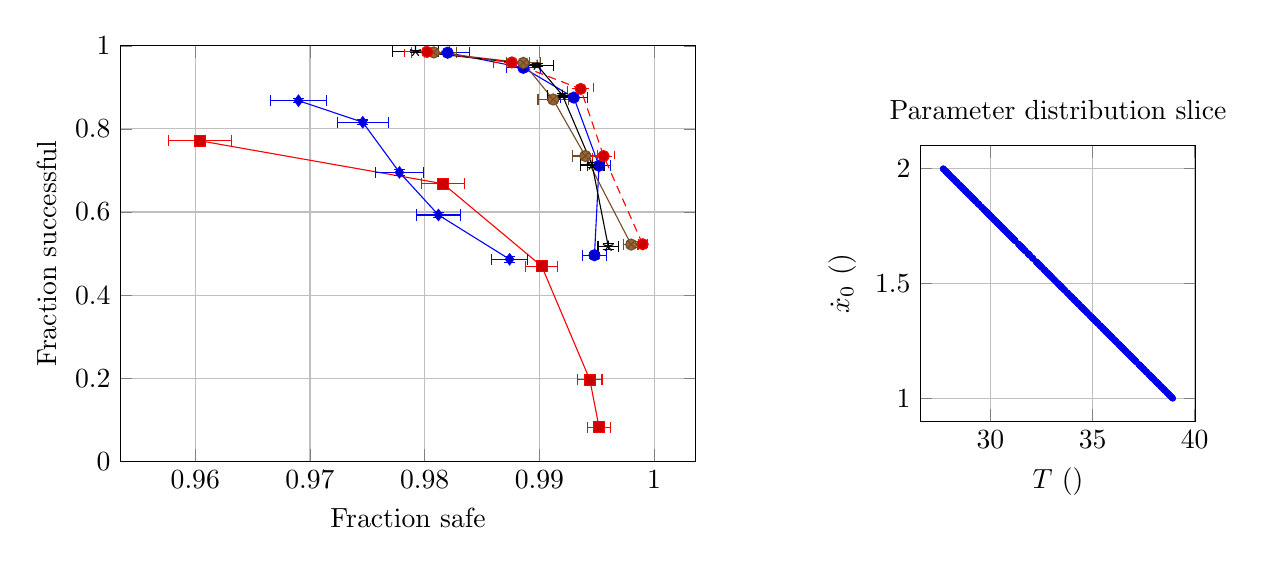
\begin{tikzpicture}[]
\begin{axis}[height = {2.7in}, ylabel = {Fraction successful}, ymax = {1.0}, xlabel = {Fraction safe}, legend style={at={(0.5,1.05), font=\footnotesize}, anchor=south, font=\footnotesize}, legend columns=2, grid=both, ymin = {0.0}, width = {3.5in}]\addplot+ [
, error bars/.cd, 
x dir=both, x explicit, y dir=both, y explicit]
table [
x error plus=ex+, x error minus=ex-, y error plus=ey+, y error minus=ey-
] {
x y ex+ ex- ey+ ey-
0.982 0.9834 0.0018804008034023813 0.0018804008034023813 0.0018070808250384592 0.0018070808250384592
0.9886 0.947 0.001501485561628335 0.001501485561628335 0.0031686287320555903 0.0031686287320555903
0.993 0.8754 0.0011791853525290755 0.0011791853525290755 0.004671116768651089 0.004671116768651089
0.9952 0.7112 0.0009775393171751847 0.0009775393171751847 0.006409924291743685 0.006409924291743685
0.9948 0.496 0.0010172506867984685 0.0010172506867984685 0.0070715487243087185 0.0070715487243087185
};
\addplot+ [
, error bars/.cd, 
x dir=both, x explicit, y dir=both, y explicit]
table [
x error plus=ex+, x error minus=ex-, y error plus=ey+, y error minus=ey-
] {
x y ex+ ex- ey+ ey-
0.9604 0.7714 0.002758240304599224 0.002758240304599224 0.005939315035643325 0.005939315035643325
0.9816 0.668 0.0019007920986053178 0.0019007920986053178 0.006660636066815469 0.006660636066815469
0.9902 0.4696 0.001393262443349134 0.001393262443349134 0.007058692019532005 0.007058692019532005
0.9944 0.196 0.001055438671907578 0.001055438671907578 0.005614544026091883 0.005614544026091883
0.9952 0.0818 0.0009775393171751845 0.0009775393171751845 0.003876178137210714 0.003876178137210714
};
\addplot+ [
, error bars/.cd, 
x dir=both, x explicit, y dir=both, y explicit]
table [
x error plus=ex+, x error minus=ex-, y error plus=ey+, y error minus=ey-
] {
x y ex+ ex- ey+ ey-
0.9808 0.984 0.0019408826355761385 0.0019408826355761385 0.0017746633162313392 0.0017746633162313392
0.9886 0.959 0.0015014855616283362 0.0015014855616283362 0.002804527246188737 0.002804527246188737
0.9912 0.8708 0.001320931857513646 0.001320931857513646 0.0047440460784692095 0.0047440460784692095
0.994 0.7348 0.0010922630670866526 0.0010922630670866526 0.006243523710026526 0.006243523710026526
0.998 0.5216 0.0006318859517121704 0.0006318859517121704 0.007065173128400112 0.007065173128400112
};
\addplot+ [
, error bars/.cd, 
x dir=both, x explicit, y dir=both, y explicit]
table [
x error plus=ex+, x error minus=ex-, y error plus=ey+, y error minus=ey-
] {
x y ex+ ex- ey+ ey-
0.9792 0.9866 0.0020184862787176513 0.0020184862787176513 0.0016262278202591003 0.0016262278202591003
0.9898 0.9534 0.0014211248781102412 0.0014211248781102412 0.0029811852497117165 0.0029811852497117165
0.992 0.8814 0.0012599672628686455 0.0012599672628686455 0.004572853616511231 0.004572853616511231
0.9946 0.7132 0.001036524421601015 0.001036524421601015 0.006396665964945574 0.006396665964945574
0.996 0.5176 0.0008927258212230546 0.0008927258212230546 0.0070673925607342486 0.0070673925607342486
};
\addplot+ [
, error bars/.cd, 
x dir=both, x explicit, y dir=both, y explicit]
table [
x error plus=ex+, x error minus=ex-, y error plus=ey+, y error minus=ey-
] {
x y ex+ ex- ey+ ey-
0.969 0.868 0.002451326538909107 0.002451326538909107 0.004787461118044853 0.004787461118044853
0.9746 0.816 0.002225299618406106 0.002225299618406106 0.0054804020802667695 0.0054804020802667695
0.9778 0.6954 0.0020838187205445653 0.0020838187205445653 0.006509396473444352 0.006509396473444352
0.9812 0.5928 0.0019209502882693128 0.0019209502882693128 0.006948905630233565 0.006948905630233565
0.9874 0.4862 0.0015775759091561385 0.0015775759091561385 0.007069081013913758 0.007069081013913758
};
\addplot+ [
, error bars/.cd, 
x dir=both, x explicit, y dir=both, y explicit]
table [
x error plus=ex+, x error minus=ex-, y error plus=ey+, y error minus=ey-
] {
x y ex+ ex- ey+ ey-
0.9802 0.9854 0.0019703726738093843 0.0019703726738093843 0.0016964502906710076 0.0016964502906710076
0.9876 0.96 0.0015651638724394007 0.0015651638724394007 0.002771558461815559 0.002771558461815559
0.9936 0.8962 0.0011278574433333764 0.0011278574433333764 0.004313795749308628 0.004313795749308628
0.9956 0.7346 0.0009361107096129862 0.0009361107096129862 0.006245027467803034 0.006245027467803034
0.999 0.5224 0.0004470346384717846 0.0004470346384717846 0.007064674792655703 0.007064674792655703
};
\end{axis}
\begin{axis}[height = {2in}, ylabel = {$\dot{x}_0$ (\si{\meter\per\second})}, title = {Parameter distribution slice}, xlabel = {$T$ (\si{\second})}, xshift=4in, yshift=0.2in, grid=both, width = {2in}]\addplot+[draw=none, mark size = {1}] coordinates {
(34.86539232802926, 1.360977590761167)
(37.25453997642316, 1.14879751541535)
(29.862649745001704, 1.8052708929838626)
(35.78003712885783, 1.2797480347373151)
(38.460398493454235, 1.0417052847731587)
(34.116297923527156, 1.4275046249087784)
(37.429513102030796, 1.1332581614537482)
(37.308097935618115, 1.1440410359131334)
(29.151776908231547, 1.868403471737873)
(38.38173417425303, 1.0486914587697127)
(32.914722016524394, 1.5342165171825584)
(35.401668126626035, 1.3133509656637625)
(29.96245904152247, 1.7964068346782882)
(28.913602643638107, 1.8895557154850702)
(32.406301907384524, 1.579369279983612)
(35.935381511944286, 1.2659519083530828)
(35.97146101336711, 1.262747689754253)
(30.709244799875258, 1.7300848312721795)
(33.31016759399417, 1.4990970165191675)
(30.032871544789874, 1.7901535040151089)
(37.50338060789048, 1.126697992194451)
(32.83752244661176, 1.5410726068728458)
(27.873865119465876, 1.9818947496033856)
(38.77018373018562, 1.0141932744062503)
(36.02310650591665, 1.2581610563129084)
(30.309888055776902, 1.7655516824354436)
(38.19035903263145, 1.0656874748995158)
(35.87706991854949, 1.2711305578552854)
(36.40583696605641, 1.224170784542059)
(34.97655505380856, 1.3511052350081205)
(28.883084754514, 1.8922660075920068)
(28.463102503283533, 1.929564608944624)
(30.598859493032684, 1.7398881444908805)
(36.31006248058976, 1.2326765114929166)
(29.095256554102573, 1.8734230413763255)
(35.72672085093836, 1.2844830505383342)
(31.14574057627722, 1.6913196646290214)
(38.48187428227614, 1.0397980211122433)
(31.62478612445186, 1.6487756550220372)
(31.827332664869996, 1.630787507560391)
(29.209031609462233, 1.863318684772448)
(33.46941002040471, 1.4849547051150347)
(34.09959236329428, 1.4289882448228879)
(37.017189205687544, 1.1698766247169146)
(29.85585723575308, 1.8058741353682874)
(37.97177565242896, 1.0850998532478717)
(35.51942967854026, 1.302892568513298)
(35.67004690100699, 1.2895162610118123)
(34.065527481767525, 1.4320135451360987)
(37.63478497682274, 1.1150279771915856)
(37.4748461182196, 1.1292321387016335)
(27.795759193649456, 1.9888313327131921)
(35.48051229835464, 1.306348818973833)
(30.90340161182993, 1.7128417751483185)
(28.83077803826768, 1.8969113642746285)
(31.437667779905063, 1.6653936252304562)
(30.04291286261942, 1.789261735113728)
(28.532298456558753, 1.9234193200214251)
(32.91371070501829, 1.5343063317035264)
(36.95647059629061, 1.1752690411820064)
(28.374438905248063, 1.9374388183616282)
(28.172278603590662, 1.9553926639795147)
(30.28011915449703, 1.7681954569718445)
(36.05809454102446, 1.2550537707793554)
(30.620123283657684, 1.7379997083785361)
(35.65112849499622, 1.2911964036415435)
(31.841263551112664, 1.6295503062955004)
(35.77173224118286, 1.2804855913691955)
(36.48796869329025, 1.216876670222891)
(38.53268031335401, 1.0352859401994667)
(35.6742601171917, 1.2891420855069535)
(28.716360079135075, 1.9070728171283235)
(38.604745499438266, 1.0288858348633863)
(34.27730785836917, 1.4132053411750292)
(34.717863569400954, 1.3740796119537337)
(27.917449962337994, 1.9780239820303736)
(36.11999874941046, 1.24955606133122)
(31.869546477460425, 1.6270385011136388)
(29.709419553520128, 1.8188792581243225)
(30.22563825684722, 1.7730339025890567)
(36.34332605527102, 1.2297223751979554)
(35.633580962008615, 1.2927547991111354)
(33.96148612482701, 1.4412534525020415)
(36.90990308446681, 1.1794046994256826)
(34.08541094152379, 1.4302476961346542)
(31.93275844741066, 1.6214246494306697)
(30.139229207119623, 1.7807078856909746)
(34.6984696362458, 1.3758019861238189)
(34.003746415922656, 1.4375003183017179)
(27.811149689186788, 1.987464503624619)
(37.09598171414075, 1.1628790662397206)
(29.9909777597009, 1.7938740888365097)
(33.47029898352672, 1.4848757563475383)
(38.12887631706916, 1.0711477515924372)
(29.126387145070947, 1.8706583352512478)
(33.32635559294333, 1.4976593611950861)
(34.15078038000119, 1.4244422397867509)
(38.92444615009738, 1.0004932371139095)
(36.08405465883709, 1.252748254099726)
(29.198348926056116, 1.8642674133165082)
(38.6434588852555, 1.0254477011318384)
(37.13233039609159, 1.1596509417325407)
(35.15687947650168, 1.335090632637506)
(28.80740114178445, 1.8989874652056438)
(32.06942236402723, 1.6092875342782207)
(32.4809887241608, 1.5727363477654703)
(37.92767562598484, 1.0890163742464618)
(34.83809747010399, 1.363401645639077)
(31.16838425374177, 1.6893086808399849)
(28.969533949180523, 1.8845884592202022)
(32.43040803098002, 1.5772284164316146)
(34.435315549166724, 1.3991726865748915)
(28.78476380643039, 1.9009978857521854)
(38.23224322257723, 1.0619677422222706)
(34.47679110093645, 1.3954892450322862)
(31.71050861373078, 1.641162645316982)
(32.65182184714021, 1.5575646672166776)
(31.191309694614638, 1.6872726736576695)
(29.401198363959374, 1.8462523655453484)
(36.49226096600787, 1.2164954737115568)
(30.34362690099168, 1.7625553373897265)
(36.735504111373764, 1.1948930629330583)
(33.818041954915806, 1.4539927215882944)
(32.44569023756341, 1.5758712044792709)
(32.30611642352629, 1.5882667474665817)
(37.03048806062402, 1.168695554118648)
(27.717633357883294, 1.9957696840245742)
(36.42560889598408, 1.2224148404987498)
(30.076044859369055, 1.7863192842478635)
(29.89582283903548, 1.8023247922703838)
(38.514829945314155, 1.0368712304339116)
(31.027754752601748, 1.701797979342651)
(29.171654665706075, 1.8666381291557659)
(33.94833139646593, 1.4424217232268268)
(37.37711948984367, 1.137911235360242)
(28.115773142867116, 1.9604109109354246)
(35.28003357978352, 1.3241533232874316)
(29.820176986142236, 1.80904289643497)
(36.45023851377389, 1.2202274854552495)
(31.885154930503358, 1.6256523152306075)
(35.79464121324775, 1.2784510467808392)
(31.103133366028967, 1.695103608700802)
(35.16200442319106, 1.3346354863951102)
(34.169491609809654, 1.422780496464507)
(30.692936270037002, 1.731533190938099)
(30.399594944280814, 1.7575848184475296)
(34.43469781331123, 1.3992275476633007)
(32.232249240320144, 1.594826888071035)
(33.6135066101293, 1.4721574946599199)
(36.29983168484421, 1.2335851079179208)
(32.61515335199505, 1.5608211943166028)
(28.22971378398156, 1.9502918486694882)
(37.097411455267064, 1.1627520910064773)
(29.96070834020587, 1.796562314368928)
(34.31965555283516, 1.409444444686043)
(31.17312320058818, 1.6888878152230746)
(37.54043012978498, 1.1234076261292203)
(36.12637806411503, 1.2489895147322354)
(28.785015274697827, 1.900975552868754)
(35.008683138374714, 1.348251941529777)
(30.499029571780515, 1.7487540344777517)
(29.54939034475698, 1.8330914436272665)
(32.329028467686406, 1.586231930045612)
(31.91269555638355, 1.6232064337137166)
(33.94010203502885, 1.4431525723775442)
(34.101802027548096, 1.4287920046582507)
(32.360161185945046, 1.5834670349959996)
(32.88544193516474, 1.5368168796478916)
(28.991655846960946, 1.8826238146571095)
(27.856513980607456, 1.9834357033208296)
(37.49915432983302, 1.1270733277235327)
(29.645325765412725, 1.8245714240308413)
(37.64779243087802, 1.1138727858900512)
(34.94865656372175, 1.3535828984261322)
(38.541895216166395, 1.0344675651717234)
(30.787861344313363, 1.72310290014979)
(30.702574749059853, 1.7306771981296754)
(30.85273551751126, 1.717341428284968)
(30.91170946069627, 1.712103955533191)
(31.67123249851894, 1.6446507550160798)
(36.896863453573395, 1.1805627483504975)
(30.442863139063704, 1.753742172374449)
(35.50229204268144, 1.3044145610407245)
(35.35913743274703, 1.3171281143208673)
(38.699507141574244, 1.0204700584747561)
(30.529353519558693, 1.7460609662914126)
(37.343335125242284, 1.1409116229802592)
(30.567696819442865, 1.7426556998718592)
(34.23045946267025, 1.4173659447006886)
(28.324426715497832, 1.9418803982683985)
(31.197907528702867, 1.686686720363866)
(32.82345213718149, 1.5423221903035977)
(28.099472879651426, 1.961858536443035)
(37.75778007010942, 1.1041047895107086)
(32.968635143795474, 1.5294284952224266)
(33.452105808887154, 1.486491491217837)
(36.45215234319151, 1.2200575183666513)
(29.876479338259216, 1.8040426875435864)
(30.303215112607557, 1.766144306162739)
(29.575577595957498, 1.8307657552435614)
(36.99296327947897, 1.1720281279325955)
(36.3258602185382, 1.2312735152275132)
(30.55142044243862, 1.7441012040463035)
(35.38639423360075, 1.314707439289454)
(38.80291418002392, 1.0112864849001848)
(35.84405372879665, 1.2740627239079352)
(28.17592188156538, 1.9550691046567157)
(30.16615857910356, 1.7783162896000388)
(28.65425652328753, 1.9125882306138962)
(35.49679713411631, 1.304902563577592)
(28.575568597941654, 1.919576501070901)
(29.399551585425396, 1.846398615859201)
(31.888990161003363, 1.6253117086142659)
(34.33452512262951, 1.4081238789849457)
(32.67261307905684, 1.5557181990180426)
(35.52941027906436, 1.3020061919125792)
(30.3040949956339, 1.766066163798055)
(37.037054846033776, 1.1681123582563255)
(36.729313535191764, 1.1954428476739107)
(32.40889376794403, 1.5791390969854322)
(28.52737943723241, 1.923856177865683)
(35.60051309392488, 1.2956915547135983)
(31.06923698266759, 1.6981139447009244)
(34.32587360904468, 1.4088922194454108)
(29.179195003142777, 1.8659684721898067)
(29.902016996572943, 1.801774689469543)
(28.756994228291003, 1.9034641005070156)
(35.660843766931094, 1.2903335908586946)
(29.927631388284137, 1.7994998767065598)
(28.20096774425927, 1.9528447829254643)
(30.379655163347074, 1.7593556693297447)
(32.69360351353164, 1.5538540396508307)
(29.305027341816167, 1.8547933088973207)
(34.62997412875683, 1.3818850684940647)
(32.03143509581517, 1.6126611815439456)
(36.955442198115506, 1.1753603731691382)
(30.048337419370736, 1.7887799805176965)
(29.4259580184821, 1.8440534619465274)
(27.9049425523228, 1.9791347644473531)
(28.278374741830632, 1.9459702715958584)
(28.767736884914726, 1.9025100457446955)
(38.52653340143526, 1.0358318471194263)
(38.09776640641769, 1.073910621099672)
(30.40145413488293, 1.7574197038292245)
(36.36880809396813, 1.2274593166991008)
(34.532735347043754, 1.39052083951654)
(31.084167545702805, 1.6967879621933566)
(34.77087263204597, 1.369371879924869)
(38.262556714381866, 1.0592756026303847)
(35.261500098673565, 1.3257992807572319)
(31.577992399333954, 1.6529314032563094)
(27.812977872690826, 1.987302142745042)
(29.408235498709203, 1.8456273979831967)
(38.659379956956045, 1.024033751602483)
(30.0756819646289, 1.7863515129103997)
(33.43473420223392, 1.488034262679048)
(31.525005422372587, 1.657637173856786)
(30.410435468881197, 1.7566220720354175)
(31.519518587879702, 1.6581244593357278)
(28.583198919012755, 1.9188988526631654)
(35.05238007716233, 1.3443712187244818)
(35.89661982461706, 1.2693943317391594)
(30.308611456650297, 1.7656650571358525)
(30.34016052415781, 1.7628631861316333)
(28.010074730595765, 1.9697979812970012)
(27.713712301721877, 1.9961179128133324)
(29.720536240024664, 1.817891985788218)
(29.031893991115187, 1.8790502672188998)
(33.55165874506173, 1.4776502002609473)
(30.9548441881701, 1.7082731626847159)
(35.088695211312164, 1.3411460735957224)
(33.00360272255805, 1.5263230264158034)
(32.25960714167061, 1.5923972343098927)
(28.78707292457783, 1.9007928130925549)
(36.678512366223444, 1.199954496782998)
(35.378637952867294, 1.3153962741680914)
(36.62871852848804, 1.2043766848589668)
(31.866483533735327, 1.6273105209826528)
(28.35805972129235, 1.9388934528159547)
(38.23130281286923, 1.0620512599583274)
(35.68727819295684, 1.287985950891933)
(29.927639546489594, 1.7994991521767678)
(37.60533010467793, 1.1176438628172347)
(35.615944921044786, 1.2943210549693795)
(28.591639388321372, 1.9181492550336257)
(38.88569934929117, 1.0039343384288482)
(28.79497991082048, 1.9000905940656767)
(32.410314088253386, 1.5790129584144417)
(33.96577776701579, 1.4408723119879405)
(32.75282640088858, 1.5485944581804099)
(36.17055071997211, 1.2450665435193509)
(33.77009979372878, 1.4582504623686694)
(33.04906747838783, 1.5222853038731938)
(35.180138811910844, 1.3330249722992142)
(34.259074726367395, 1.414824624656537)
(35.95209634100341, 1.2644674652750074)
(32.52756419210297, 1.5685999829393455)
(32.290520428752544, 1.5896518269313906)
(30.217544868712395, 1.7737526759580466)
(38.028544082560195, 1.0800582519928776)
(33.10363760900518, 1.5174389334808893)
(30.866737577419656, 1.7160979060906165)
(37.38234512804077, 1.1374471467104112)
(36.79066074201051, 1.1899946055052835)
(30.414217975336317, 1.7562861478386929)
(28.475285680743404, 1.928482621603605)
(30.389493557819872, 1.7584819220408638)
(34.5880119982344, 1.385611723069769)
(37.28751623752607, 1.1458688954239726)
(38.19444693152643, 1.0653244288164805)
(37.855949473634, 1.0953863700147426)
(30.858059509381768, 1.716868604850642)
(30.471136863069006, 1.7512311844521307)
(30.614807611324114, 1.7384717929552296)
(38.01497606343814, 1.0812632270481224)
(34.71723500936517, 1.3741354343370187)
(35.534395432748774, 1.3015634606795048)
(38.146980052107466, 1.06953995984836)
(36.602411133918864, 1.2067130431688395)
(36.75261407010479, 1.1933735284098765)
(30.68848585079928, 1.7319284324334563)
(29.231283881116497, 1.861342461712567)
(29.94656969119199, 1.797817967034459)
(36.605451649594535, 1.2064430151337002)
(31.201938569993022, 1.6863287238016853)
(28.516704584294985, 1.9248042109862358)
(29.26653603920365, 1.858211719431292)
(28.976401650881368, 1.883978538998102)
(27.691415467338263, 1.9980980934868326)
(35.21926940216246, 1.32954978666408)
(32.61793696939982, 1.5605739814032131)
(34.29330720472395, 1.4117844400778015)
(36.435523654939175, 1.2215343112842652)
(37.13431920206337, 1.159474315980163)
(27.869530778392917, 1.9822796822031157)
(35.027749323117234, 1.3465586746787532)
(28.91974009428083, 1.88901064882053)
(29.873967008245526, 1.8042658074382303)
(36.774391734284215, 1.1914394552145455)
(28.646811220014513, 1.9132494476008424)
(36.8616660240591, 1.1836886301901335)
(35.53043850795398, 1.301914874959682)
(33.24900371180081, 1.5045289776375832)
(27.955098394950703, 1.974680426736172)
(28.712943362076068, 1.907376255588271)
(29.829774862819537, 1.808190509518691)
(36.25137588648968, 1.2378884647877724)
(31.483172651593588, 1.6613523400005694)
(31.70804448380833, 1.6413814845640915)
(29.424762578410242, 1.844159628915609)
(38.343387292941614, 1.052097043255629)
(29.82768137954139, 1.80837643165707)
(29.810045942956027, 1.809942633840495)
(33.6628586153572, 1.4677745457053992)
(38.838060411556185, 1.0081651499506055)
(30.340322970620278, 1.7628487592699575)
(33.401707206590274, 1.4909673884022845)
(35.11895673599539, 1.3384585492011196)
(30.410459761804802, 1.7566199145821666)
(34.495015821477715, 1.3938707085721387)
(33.43763437797261, 1.4877766982262337)
(31.510229634681828, 1.6589494107742604)
(35.90044266429143, 1.2690548255513827)
(37.495297672547345, 1.1274158372515681)
(38.85970743405006, 1.0062426790364067)
(37.1047639887864, 1.1620991128964122)
(34.93390068646024, 1.3548933670994459)
(37.64934276453956, 1.1137351008401812)
(31.388087331441195, 1.66979686221659)
(28.390919930196624, 1.935975139414154)
(38.73189959350513, 1.0175932865448374)
(28.50477720824467, 1.9258634806177026)
(38.443972846084236, 1.0431640456408315)
(36.17868800747418, 1.2443438714498953)
(36.853072540044685, 1.1844518170475413)
(38.18550678532188, 1.0661184027245223)
(31.51265282131704, 1.658734207698309)
(34.62671449619698, 1.3821745562880123)
(38.12569020611266, 1.0714307099367086)
(35.95242000937654, 1.2644387203040375)
(33.99731117304062, 1.4380718318791632)
(38.72593223044635, 1.0181232477401114)
(30.75568887159735, 1.7259601357373577)
(36.46014911692935, 1.219347325317109)
(36.121180196771576, 1.249451137054034)
(37.8134234077868, 1.0991631076565895)
(36.867389619784134, 1.18318031795878)
(28.334455414335658, 1.940989750059)
(31.548459271163896, 1.655554238795391)
(33.93604155849933, 1.443513183081764)
(36.853667363603876, 1.1843989907989456)
(28.20056621083139, 1.9528804430877982)
(33.75459795787456, 1.4596271795848523)
(33.39866913143499, 1.4912371996949385)
(29.80783224632634, 1.8101392321202185)
(36.36935904060226, 1.227410387157881)
(29.38348038477232, 1.8478258983328313)
(36.56567976949976, 1.209975153685634)
(32.281007425606845, 1.59049667623385)
(35.044440793052765, 1.3450763061232)
(31.006122421848993, 1.7037191454841036)
(29.40289669744131, 1.8461015366393152)
(29.738508532584188, 1.8162958674436775)
(36.8891435005381, 1.1812483569681975)
(27.970853445620342, 1.9732812215257243)
(37.307857823156, 1.1440623602880997)
(33.58745139609215, 1.474471456830182)
(31.000025533815688, 1.7042606097854627)
(31.573966697799996, 1.653288925595027)
(38.37529868292304, 1.0492629944118081)
(37.905405020669825, 1.0909942255177776)
(37.34887204454711, 1.1404198894718378)
(30.656524568770305, 1.734766912187362)
(29.114002310957986, 1.8717582317088821)
(35.58604805845764, 1.2969761937426605)
(32.77920192728552, 1.5462520490865435)
(35.63053382959022, 1.2930254147788438)
(29.811954488552576, 1.809773136007764)
(32.085420857153224, 1.6078667089561964)
(36.392571541531304, 1.2253488861872732)
(31.1194307895222, 1.6936562353887918)
(35.24033578833744, 1.3276788820304226)
(35.52607940373205, 1.3023020067733528)
(36.642258390782835, 1.2031742104100502)
(35.74157731072127, 1.2831636491366547)
(36.499922726728656, 1.2158150331502084)
(34.538984682506324, 1.3899658363671112)
(32.50444253071668, 1.5706534164550014)
(36.84124754231708, 1.185501994465624)
(32.80902349627011, 1.5436035971340936)
(28.77969156833691, 1.9014483509469882)
(37.92205849431317, 1.0895152314109084)
(35.8653991662795, 1.2721670367424953)
(34.55337920192635, 1.3886874598644452)
(38.10963831648011, 1.072856277399635)
(35.61441412884893, 1.2944570045427237)
(33.388664903205516, 1.492125674670913)
(28.61306542582029, 1.916246409785054)
(31.364625881958926, 1.6718804722949443)
(33.32345041838838, 1.497917369592506)
(33.185892002059155, 1.510133925216771)
(30.923767245660397, 1.7110331042930373)
(37.06593335390926, 1.165547659510723)
(27.686587468916706, 1.9985268677693866)
(30.186553613854027, 1.776505007650619)
(37.84089921810841, 1.0967229824060025)
(36.54837180950304, 1.2115122726906713)
(35.88728068959226, 1.2702237398230676)
(29.45870010248062, 1.8411456392113124)
(29.75483024954277, 1.8148463366303043)
(30.610525579182962, 1.738852080001513)
(38.38227926023941, 1.0486430497123083)
(38.51410794792414, 1.0369353509836468)
(37.90375729256117, 1.0911405601633064)
(35.238024139791435, 1.3278841794146148)
(34.92769689511185, 1.355444325478521)
(30.595670104975508, 1.7401713938742887)
(28.055656655130967, 1.9657498530079067)
(31.077014589013206, 1.6974232158958076)
(31.590515106922194, 1.6518192622626826)
(29.14586394878097, 1.868928601351601)
(33.77957274997793, 1.4574091696289584)
(28.661101691433583, 1.9119803115955964)
(37.77619596707193, 1.1024692746827771)
(35.78784852305089, 1.2790543052352672)
(37.31331813987255, 1.1435774298514612)
(35.669504847601885, 1.2895644007458362)
(38.87602171546993, 1.00479380857283)
(27.846659645659393, 1.9843108662824693)
(33.47106701107338, 1.4848075478620444)
(34.43629099592625, 1.399086057200155)
(31.453124307661557, 1.664020931824018)
(29.66689777763254, 1.8226556147750852)
(38.70722144716564, 1.0197849514062487)
(28.306139007290597, 1.9435045286598047)
(30.80637635837249, 1.7214585827377895)
(31.502649917743923, 1.6596225650316232)
(29.264264102604468, 1.8584134899996032)
(32.647260054688545, 1.5579697997612303)
(34.0978630923447, 1.4291418212837743)
(37.61566577969445, 1.1167259520697645)
(33.462670423948616, 1.4855532483171745)
(37.910767246753366, 1.09051800650503)
(29.065817378613545, 1.8760375329828112)
(31.835722630959946, 1.63004239511901)
(35.40084604704941, 1.313423974507157)
(38.330373363779216, 1.0532528096110818)
(27.95342840469799, 1.9748287384815282)
(33.874043022569424, 1.4490192697540476)
(38.19537644195401, 1.065241879044937)
(32.260204351428044, 1.5923441961431577)
(33.49780738392162, 1.4824327367742791)
(36.76247141215121, 1.1924980983879923)
(32.92199616838547, 1.5335705001433861)
(37.745252873871394, 1.105217329141084)
(28.63997702666097, 1.9138563919484042)
(31.193100934101977, 1.687113593774247)
(36.26777445586846, 1.2364321087150565)
(33.14375662114745, 1.513875966150315)
(30.475355491626967, 1.750856528274692)
};
\end{axis}

\end{tikzpicture}

        \vspace{-1em}
        \caption{Scenario 2: Fully correlated ($\rho=1$)} \label{fig:100}
        \vspace{1em}
    \end{subfigure}
    \caption[Performance curves at correlation extremes]{Approximate Pareto performance curves for model distributions at correlation extremes. The scatter plots at right illustrate the level of correlation with samples from the joint parameter distribution. Error bars indicate the standard error of the mean.}
    \label{fig:gaps}
\end{figure}

\begin{figure}[htbp]
    \centering
    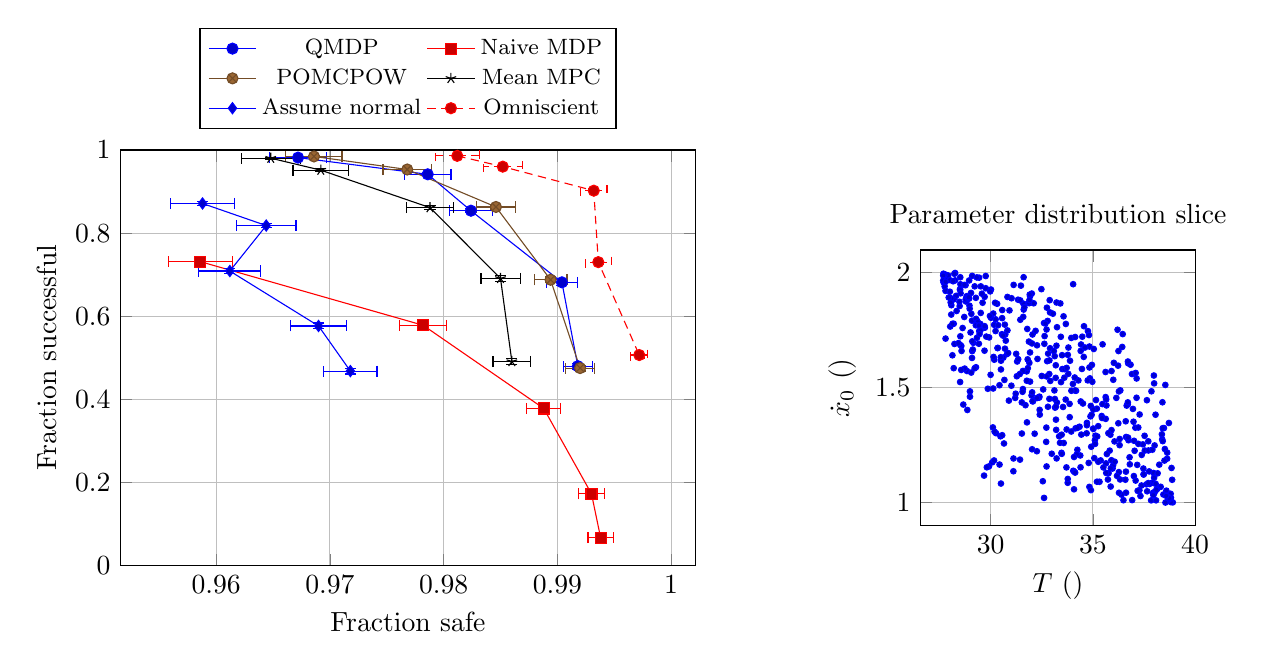
\begin{tikzpicture}[]
\begin{axis}[height = {2.7in}, ylabel = {Fraction successful}, ymax = {1.0}, xlabel = {Fraction safe}, legend style={at={(0.5,1.05), font=\footnotesize}, anchor=south, font=\footnotesize}, legend columns=2, grid=both, ymin = {0.0}, width = {3.5in}]\addplot+ [
, error bars/.cd, 
x dir=both, x explicit, y dir=both, y explicit]
table [
x error plus=ex+, x error minus=ex-, y error plus=ey+, y error minus=ey-
] {
x y ex+ ex- ey+ ey-
0.9672 0.9818 0.002519146923115848 0.002519146923115848 0.0018906260585791856 0.0018906260585791856
0.9786 0.9416 0.002046764727361175 0.002046764727361175 0.0033166380594818385 0.0033166380594818385
0.9824 0.854 0.0018597687350715502 0.0018597687350715502 0.004994175443220966 0.004994175443220966
0.9904 0.6816 0.0013791114493317603 0.0013791114493317603 0.006588851993641919 0.006588851993641919
0.9918 0.4798 0.001275491033082978 0.001275491033082978 0.007066001533790888 0.007066001533790888
};
\addlegendentry{QMDP}
\addplot+ [
, error bars/.cd, 
x dir=both, x explicit, y dir=both, y explicit]
table [
x error plus=ex+, x error minus=ex-, y error plus=ey+, y error minus=ey-
] {
x y ex+ ex- ey+ ey-
0.9586 0.7314 0.0028175868680755584 0.0028175868680755584 0.006268864947783357 0.006268864947783357
0.9782 0.5782 0.0020653825701385745 0.0020653825701385745 0.006984748337761956 0.006984748337761956
0.9888 0.378 0.0014884068902736884 0.0014884068902736884 0.006858032263069643 0.006858032263069643
0.993 0.1726 0.0011791853525290779 0.0011791853525290779 0.005344863095749249 0.005344863095749249
0.9938 0.0672 0.0011102065175913607 0.0011102065175913607 0.0035410930329452914 0.0035410930329452914
};
\addlegendentry{Naive MDP}
\addplot+ [
, error bars/.cd, 
x dir=both, x explicit, y dir=both, y explicit]
table [
x error plus=ex+, x error minus=ex-, y error plus=ey+, y error minus=ey-
] {
x y ex+ ex- ey+ ey-
0.9686 0.9846 0.002466581603142498 0.002466581603142498 0.001741601169879885 0.001741601169879885
0.9768 0.9532 0.002129145051829554 0.002129145051829554 0.0029872624168876577 0.0029872624168876577
0.9846 0.863 0.001741601169879886 0.001741601169879886 0.0048632222020011835 0.0048632222020011835
0.9894 0.6878 0.0014484293526154162 0.0014484293526154162 0.006553992902391117 0.006553992902391117
0.992 0.4752 0.0012599672628686458 0.0012599672628686458 0.0070630708189765926 0.0070630708189765926
};
\addlegendentry{POMCPOW}
\addplot+ [
, error bars/.cd, 
x dir=both, x explicit, y dir=both, y explicit]
table [
x error plus=ex+, x error minus=ex-, y error plus=ey+, y error minus=ey-
] {
x y ex+ ex- ey+ ey-
0.9648 0.9804 0.0026064440738565783 0.0026064440738565783 0.0019605960285988197 0.0019605960285988197
0.9692 0.9516 0.002443658383092597 0.002443658383092597 0.003035346877398558 0.003035346877398558
0.9788 0.8614 0.002037386116679335 0.002037386116679335 0.004887001591662435 0.004887001591662435
0.985 0.691 0.0017191832706909644 0.0017191832706909644 0.006535468037447208 0.006535468037447208
0.986 0.491 0.0016617317083254108 0.0016617317083254108 0.00707062930436548 0.00707062930436548
};
\addlegendentry{Mean MPC}
\addplot+ [
, error bars/.cd, 
x dir=both, x explicit, y dir=both, y explicit]
table [
x error plus=ex+, x error minus=ex-, y error plus=ey+, y error minus=ey-
] {
x y ex+ ex- ey+ ey-
0.9588 0.8714 0.0028110660644111002 0.0028110660644111002 0.004734647967724278 0.004734647967724278
0.9644 0.8182 0.0026206681553214727 0.0026206681553214727 0.005454878838308729 0.005454878838308729
0.9612 0.7088 0.0027313740279969255 0.0027313740279969255 0.00642563380173123 0.00642563380173123
0.969 0.5766 0.0024513265389091076 0.0024513265389091076 0.0069882941588809795 0.0069882941588809795
0.9718 0.468 0.002341377459890212 0.002341377459890212 0.007057277168441554 0.007057277168441554
};
\addlegendentry{Assume normal}
\addplot+ [
, error bars/.cd, 
x dir=both, x explicit, y dir=both, y explicit]
table [
x error plus=ex+, x error minus=ex-, y error plus=ey+, y error minus=ey-
] {
x y ex+ ex- ey+ ey-
0.9812 0.986 0.0019209502882693128 0.0019209502882693128 0.0016617317083254147 0.0016617317083254147
0.9852 0.96 0.001707856948070012 0.001707856948070012 0.0027715584618155584 0.0027715584618155584
0.9932 0.9022 0.0011623348073773246 0.0011623348073773246 0.004201257206173249 0.004201257206173249
0.9936 0.7302 0.0011278574433333766 0.0011278574433333766 0.006277696543699677 0.006277696543699677
0.9972 0.5066 0.0007473578184121366 0.0007473578184121366 0.007071158904850855 0.007071158904850855
};
\addlegendentry{Omniscient}
\end{axis}
\begin{axis}[height = {2in}, ylabel = {$\dot{x}_0$ (\si{\meter\per\second})}, title = {Parameter distribution slice}, xlabel = {$T$ (\si{\second})}, xshift=4in, yshift=0.2in, grid=both, width = {2in}]\addplot+[draw=none, mark size = {1}] coordinates {
(32.869304905930726, 1.4513325359526805)
(29.913387126609045, 1.1578294322776839)
(32.98601730058539, 1.2128001839154339)
(27.827263524121463, 1.97411476133106)
(30.42922629204157, 1.5106234514357078)
(29.81018855833017, 1.1539392792095646)
(29.012682005279917, 1.739987887736106)
(31.760357869558295, 1.5705512217762632)
(32.73201773045523, 1.157576247194449)
(28.072760440895294, 1.8582508600976713)
(35.85707313265573, 1.2954812104520939)
(28.517227677105065, 1.9492122574534105)
(34.289976962037194, 1.531411432369081)
(30.256213494647593, 1.3022780343221076)
(38.54458120770039, 1.5117727197772561)
(30.475333478262048, 1.2885876968025678)
(31.43218766975735, 1.1872153009389692)
(37.27613143469245, 1.0544114496448302)
(32.903108142625314, 1.826769513556009)
(28.785879115987175, 1.8742926602873808)
(29.702314399981166, 1.89475064185839)
(37.54080620883958, 1.226712181050568)
(35.6632992326432, 1.4226762524985381)
(33.34913815738645, 1.28855138277302)
(33.22094053440928, 1.869977318316502)
(35.99638973353763, 1.5342075305567173)
(34.951961209502784, 1.598897455426171)
(38.52109271353686, 1.2333705059445588)
(30.81741489942729, 1.8941264337482977)
(32.76144494706677, 1.615101328635862)
(29.993602756031922, 1.5557722740324473)
(34.82729427802621, 1.6786398408065217)
(31.119803875982946, 1.946479842735128)
(34.24011170339607, 1.2300664463661648)
(33.238501459062576, 1.4356106957626436)
(36.84265332938331, 1.5996147045951756)
(37.751230455202624, 1.1359815967222824)
(36.72646331405861, 1.6057347909495177)
(34.420296181807124, 1.6875666945999852)
(32.39323385324527, 1.4035030810482814)
(28.498258964223115, 1.9281260954798247)
(37.37913944112536, 1.0749434697145486)
(34.38127496478189, 1.20530690289752)
(30.24011940303437, 1.7969150039583075)
(31.57420057258384, 1.4938007305013592)
(28.836160287926702, 1.5724479778537188)
(33.676312883209846, 1.7767707455193098)
(27.80675383409372, 1.990645975374731)
(33.438926369479084, 1.5241027160094827)
(33.18404662652679, 1.5972717306545479)
(36.70770670180134, 1.4276265903539043)
(35.90467704593999, 1.1846213281714504)
(36.91259817758802, 1.5591772110173383)
(36.20609087929939, 1.7516814970971353)
(36.27155677629613, 1.1330270425716205)
(36.740020556336006, 1.2716234185742046)
(31.33752212592271, 1.8821565551735662)
(28.125061989519782, 1.6406181699913807)
(32.549396934151225, 1.093369738636796)
(32.71310774588132, 1.2644271131486486)
(29.32646475996489, 1.7168299017930027)
(28.30713917745935, 1.8988945138204958)
(37.71492512270662, 1.227056207920398)
(33.704887870584145, 1.153498295393798)
(37.952643916380765, 1.0437862617095104)
(35.962125258375934, 1.1485457851342111)
(31.447116728561852, 1.7949979425865707)
(31.926077031135975, 1.8974565525245195)
(28.25890921753333, 1.998271167424189)
(36.30836331971451, 1.2770785497197026)
(29.493359443246277, 1.7769787822286882)
(37.18891211645412, 1.0516056004092276)
(28.2589247114842, 1.9662754792365487)
(28.771855481429792, 1.8830056435977416)
(38.403058138650195, 1.4364830455862)
(28.18395696037629, 1.8832393657594335)
(30.332045781289953, 1.672042557910659)
(33.191498959790216, 1.3609150667531675)
(38.908097199151534, 1.0015587109139685)
(28.959474425723624, 1.856238152704364)
(38.754939363451086, 1.032929820014969)
(38.317523661112844, 1.0690943228206555)
(31.86729567863654, 1.7001862128866079)
(37.32636484872495, 1.0292127108933509)
(28.98431054686438, 1.4605940442638436)
(31.27648283986079, 1.5495017832411266)
(37.709956091802766, 1.2668521351989743)
(33.53813650706997, 1.4161099087759976)
(33.50322614106741, 1.5807934374509411)
(35.429804785825425, 1.3767890606513797)
(29.083233297741828, 1.7911162115804729)
(30.431173906772585, 1.1657651366734787)
(37.84965343868909, 1.0102968425640697)
(38.71835213561202, 1.3464782100349835)
(30.16520851064251, 1.7729712588050723)
(34.210856239458764, 1.2104357676656856)
(35.25838563475642, 1.3326864693801073)
(36.34172167578728, 1.4883113580740828)
(33.473229844612426, 1.2956598046214594)
(29.09248446963431, 1.9856546618721471)
(30.49900755440912, 1.5791101186212488)
(29.31792683812452, 1.7918333458686235)
(36.95919547580425, 1.4076630651525792)
(37.090373534143616, 1.0963289695801741)
(33.42948004420784, 1.7209911045969917)
(29.420155325939234, 1.690716963912365)
(32.78435599562294, 1.7899803935585255)
(38.01998963932212, 1.2489338290686025)
(28.768383948745782, 1.9452473132277077)
(34.03848437876062, 1.138792245429098)
(31.773596021467966, 1.3491962132422954)
(28.22440213930195, 1.689848845968528)
(30.074248719198906, 1.1755662976045174)
(37.642205067249485, 1.4454700978710495)
(31.59701697228397, 1.8648417389610623)
(32.02369519817464, 1.2322084789768204)
(34.174545619825494, 1.486325433288812)
(36.80782934399372, 1.1667658208172715)
(35.627561275651075, 1.3643523342334127)
(34.433009425242474, 1.296046541706918)
(28.501995496992226, 1.5244741023690547)
(31.60969494923184, 1.9797353073867057)
(32.63568139838084, 1.7240347795328435)
(36.65309981501119, 1.4220543877165983)
(28.94298790002817, 1.887088923785505)
(35.98876596787989, 1.1623127401241138)
(32.3672097669625, 1.4566002146717074)
(28.57180313626573, 1.659346786925485)
(37.98359578965501, 1.5526729610062573)
(31.52224178949576, 1.3006354608224773)
(33.94176120116501, 1.7160587702389936)
(34.15168182111772, 1.3234119377443234)
(29.712703859561667, 1.7605878708222582)
(30.10568691932891, 1.3272745960108723)
(27.691680151392386, 1.9577339174471318)
(37.91026455962238, 1.2303944394505857)
(30.64849795190202, 1.2574554352434086)
(37.28591080558049, 1.3834280907430783)
(33.49245869053544, 1.6411977631196741)
(28.220249460390807, 1.9947659792394465)
(32.86405711758786, 1.559205349625167)
(28.016734451181534, 1.7655684420776983)
(36.623461518162685, 1.2855014270697416)
(29.432153616463715, 1.9779355230306521)
(30.54649067844308, 1.7321723312241595)
(29.51097436605543, 1.8247701709053863)
(34.75602447972217, 1.745775761403149)
(33.40753777277332, 1.8660039195592497)
(28.076084985753976, 1.8878604964771515)
(30.916911125704218, 1.8357134483252275)
(32.0094734525281, 1.9089135641389932)
(38.81717678965353, 1.0215239071956714)
(33.24385565860047, 1.762667774313171)
(30.17303098657781, 1.6213726596920868)
(29.283885847262507, 1.799002808409155)
(28.501028416596224, 1.9244033269461434)
(33.795937255841146, 1.5598550278771492)
(34.85394352591439, 1.5404542877300573)
(27.836591179339024, 1.9771496486746254)
(27.68597075731983, 1.9950706978542951)
(30.798255085243028, 1.6460708790559193)
(30.119080009707034, 1.4963685885395448)
(33.864682415076516, 1.3717945664299998)
(36.24316608564006, 1.3452512780325137)
(34.896223260743724, 1.4207066419089558)
(31.197085450152272, 1.4554959267772731)
(28.714752184725963, 1.946613379848993)
(37.07846059796824, 1.3259914861309843)
(34.80607150109689, 1.728617411524652)
(31.998305138924305, 1.4661924384416793)
(38.81943685000936, 1.0025019679727418)
(38.658547254551124, 1.0088414483626926)
(34.084148404227605, 1.1348538582520502)
(35.149584382701136, 1.4460814146120309)
(32.399253245389595, 1.382776247001289)
(28.189316569795913, 1.777712562107288)
(30.696344288878972, 1.6694054936009444)
(30.619695814472287, 1.6307758481634593)
(35.9106476621788, 1.315505121499159)
(30.736929207034095, 1.7042848794408667)
(35.32269178518914, 1.0910654703296994)
(35.37878940226285, 1.1838891780394942)
(29.272813172383444, 1.8902300607865534)
(32.87058731847048, 1.6185478333892196)
(34.34808214432007, 1.3301206937797443)
(37.62034239967352, 1.0799333198388248)
(27.789547902110066, 1.7132109762070198)
(34.12530396608332, 1.48764924189354)
(30.50241086927492, 1.6169758231883324)
(34.70624045410622, 1.3470713451198462)
(30.138996332540845, 1.6334683605096405)
(35.91111000866624, 1.5721309971015471)
(32.7219957061864, 1.3263622313795826)
(33.13814131754188, 1.450860964697966)
(32.90443041237923, 1.6713093198430966)
(28.509474417119304, 1.9797490598144893)
(31.889889555130782, 1.8671920297656024)
(32.0659399293272, 1.440375184226922)
(38.449299690030614, 1.0356822083451358)
(30.31209678838252, 1.8645134956105296)
(28.038917692490116, 1.8704104578744298)
(29.366201604557823, 1.785297797472309)
(27.916444504167238, 1.987130479262211)
(38.550025080125884, 1.0007190860696629)
(34.694056085563304, 1.3016218648405888)
(32.60882044459191, 1.7808310652909225)
(29.51517083714591, 1.9401631628170062)
(27.788530631479823, 1.9205808593509845)
(37.443899583323116, 1.2535143849572954)
(32.10349985461351, 1.866492432815056)
(38.06446697680346, 1.382450532688059)
(31.01135089474072, 1.5085256747809237)
(38.80549693074782, 1.0388323682796698)
(29.270957915202757, 1.7709857042299508)
(30.012126554387756, 1.9263435988803517)
(31.700527686649288, 1.4238341988278505)
(28.526163287419713, 1.9099091361054183)
(29.436156547115168, 1.7459776994095464)
(34.40185126074397, 1.659674852777882)
(31.868421195473346, 1.8686517594449836)
(38.14538031295696, 1.0598118855893084)
(29.27852224352739, 1.5888021369584007)
(28.329976365573867, 1.8331081170790742)
(34.8275650892127, 1.068796554681855)
(38.84778291647997, 1.1510203017444816)
(37.864720847606485, 1.4840797595117325)
(38.67678046700008, 1.0253970156558108)
(28.126397722399215, 1.7774021237859468)
(38.033030416991224, 1.0469255523873653)
(35.13012790781824, 1.2914815653902616)
(28.983188933032203, 1.483831319662033)
(38.87810161191858, 1.0996298508592246)
(31.294436591446136, 1.6135717408615866)
(32.60982792366024, 1.021015854463456)
(36.62035238254833, 1.0435517365072586)
(36.02559390750612, 1.6078054629538303)
(36.330820326370535, 1.1010607057914756)
(35.474199115726385, 1.6881786301157045)
(38.632386986924864, 1.1913227864812967)
(29.701465650656928, 1.7671183771953076)
(32.56640026515381, 1.4923170409777917)
(32.38258751787196, 1.4609862563901983)
(36.49447346948934, 1.0109380011941336)
(36.70937258438944, 1.4361062838933871)
(37.528736773508975, 1.2907566120522225)
(38.47719512765266, 1.3244564825390843)
(29.214910222163702, 1.9401758478341042)
(28.188228004117697, 1.5846178206086243)
(35.640853307963994, 1.171027060855362)
(28.002237011306278, 1.9672292540077914)
(33.88114766640982, 1.6168832137674802)
(30.123509432089676, 1.8220906580971818)
(30.713948204684204, 1.7317584715040364)
(30.560118436138065, 1.2933688956287357)
(28.705258729599073, 1.807017104792434)
(35.61954411888624, 1.5679872511195645)
(31.894687148873796, 1.8805662715243523)
(34.0227822583743, 1.5162603842603284)
(36.250217109745634, 1.6591230418389082)
(28.000038215710383, 1.91682011261704)
(38.766121402939206, 1.01657423331434)
(34.03274392512658, 1.9495456753478142)
(33.14968298672305, 1.413134543325225)
(32.479554022161615, 1.927989247990386)
(30.011714496829892, 1.8035457084625472)
(33.463753268654735, 1.216729158717434)
(34.61114178508798, 1.6743367827176185)
(28.657752571489507, 1.4265568672266382)
(36.40282241755396, 1.035093101636605)
(34.82956788008441, 1.5877172737824694)
(34.07525755523877, 1.0582485410785367)
(33.21585609500974, 1.682311704880207)
(33.56301880303135, 1.8098846251244223)
(31.61344751614734, 1.8392368945737516)
(29.601570603315523, 1.8690039352108736)
(36.7942989509319, 1.1973393696741175)
(37.041064823179454, 1.2257241456621804)
(38.41407536738082, 1.3235748492303068)
(36.30683993174727, 1.2501351967573076)
(36.58943609952783, 1.1000313576487561)
(38.63470038260333, 1.217780820883205)
(31.925348988483062, 1.526237380072249)
(29.566132175155985, 1.908197651012379)
(29.695883504401742, 1.6606571192154935)
(27.734807383711846, 1.9884585044709717)
(29.673408603169996, 1.117803053008504)
(37.168941003962885, 1.1644519741243982)
(31.908544238713038, 1.9042384547742577)
(37.922610223726394, 1.0875321795690256)
(31.476723415666342, 1.9432961152149117)
(28.819617328318596, 1.8971742828297717)
(30.21417256263376, 1.8687472241241831)
(29.083491688809715, 1.6291346623450016)
(37.013501749013095, 1.269075011174467)
(29.04660827355744, 1.5655922164623624)
(33.767152418623986, 1.086586799780014)
(37.96838864484911, 1.1292063616613806)
(33.47673659690291, 1.21244044091716)
(28.067970320933508, 1.8176229834385997)
(31.01966536475208, 1.888420085853403)
(29.09318118302773, 1.6588263872006845)
(37.22334312850211, 1.2557928551225501)
(30.60307713200404, 1.7258958551092962)
(37.97010505224967, 1.0373477653946672)
(36.921117924722324, 1.0113327669785157)
(29.211515156930865, 1.5840214255159664)
(29.50139315893612, 1.749662293737309)
(34.24066579058693, 1.3253021950412056)
(28.868898885554543, 1.8906086462936489)
(28.724412659810337, 1.582783199064156)
(35.44519348549866, 1.3683122085157935)
(30.499075270135517, 1.0832915812409134)
(32.73239731259096, 1.7526859576891711)
(29.92096060188384, 1.7183419462302778)
(30.562650958562863, 1.8371667167497736)
(32.26473558139569, 1.6839531348464867)
(29.453860199628433, 1.7331814467900457)
(36.23166268516234, 1.5955960936645273)
(34.4026123526991, 1.4399813810925717)
(33.609980878511166, 1.5803450436547384)
(29.7561497298861, 1.9319351829470066)
(32.14857380147146, 1.299915653969196)
(31.59024656870645, 1.807764990359165)
(35.26235608010798, 1.177916628447929)
(34.13033345839828, 1.7200785141431585)
(29.781638717742837, 1.7219018816664187)
(35.193059147980584, 1.4088682093949134)
(37.38883245103652, 1.207794342489831)
(28.944248744779905, 1.965812251451129)
(36.71267990595521, 1.6135493078727432)
(37.094214907053356, 1.5639191422959502)
(30.490165346325348, 1.6321970646692663)
(30.23656313342251, 1.7459848678866503)
(30.188001596312276, 1.3084368552060754)
(33.60154169502378, 1.54323144993298)
(29.857015467317975, 1.495165951457135)
(27.67589311300954, 1.9869552449803227)
(36.61566364950632, 1.135037356855897)
(31.650553295981016, 1.8491099586677238)
(32.25791732113888, 1.2237763573565497)
(31.442121273341225, 1.8793509436102682)
(31.1136096024152, 1.1923165532771065)
(35.76698358531913, 1.1283560183636352)
(37.220153661339445, 1.326870713245261)
(33.714043973038955, 1.3183262379196117)
(29.035545940340732, 1.9116745720706885)
(35.734455148559825, 1.1008334139845688)
(31.890581558393215, 1.6078071832154088)
(33.08787401698906, 1.6589614552824254)
(35.09507626598807, 1.2717499838212825)
(28.8554104583114, 1.40310290401584)
(32.9148026033445, 1.5293311117823536)
(34.07716624108215, 1.1987525036893298)
(37.78105972117159, 1.0817955447086331)
(34.917795114107946, 1.2431862332848205)
(31.221262545798684, 1.4736962685207529)
(32.73823551055381, 1.5486379863690938)
(28.47918111546346, 1.8546853735200488)
(34.70511877954181, 1.3366914707010553)
(29.422527153270604, 1.7701286070566589)
(34.88068994409318, 1.3752796607458662)
(35.65172815268501, 1.1293301247311134)
(33.77302939015061, 1.6424652925392738)
(32.74870913341253, 1.8473771681197508)
(37.95679051812136, 1.0328341200407731)
(32.49610873930395, 1.5507469103550802)
(34.47997814709608, 1.7214659143788937)
(35.62336007671036, 1.4590340332764289)
(32.026276711192615, 1.4796060773824613)
(31.557438713430955, 1.4820310269541803)
(36.272987398139264, 1.4835513577572292)
(36.277464648936714, 1.0432373176727687)
(34.1094309903091, 1.5441840591533904)
(38.07104700214251, 1.0819624036068511)
(31.924316825931193, 1.653021866124452)
(30.66878974036207, 1.5335747576123837)
(29.75585098322768, 1.9850838845621293)
(36.43484491251865, 1.676932794475463)
(33.18815922015791, 1.4171982483342258)
(31.816424861206517, 1.5847172105934217)
(35.19789225177901, 1.09123671779325)
(34.55190539270591, 1.6336278583706725)
(34.13181917779716, 1.1309605345911535)
(36.18019688661143, 1.1166733865280416)
(27.745056813005657, 1.9399301843440788)
(31.521028228388683, 1.4359357977930727)
(37.48504718782903, 1.1224966989482006)
(29.12290055946621, 1.665530233579497)
(36.14607120234877, 1.455549075514417)
(30.162223237556248, 1.1836930381851691)
(33.131073062156986, 1.6369065059903687)
(37.653467449421996, 1.049686546265575)
(33.20175259029157, 1.3166244348681442)
(27.94599562073544, 1.8917396373375983)
(35.512615088057785, 1.1533187776321268)
(34.39597329226231, 1.153935927661022)
(28.16021244911203, 1.962245965042433)
(32.0434957382963, 1.7309992803557948)
(29.148939866200283, 1.6947467959993134)
(36.98665325202942, 1.3519935609205542)
(33.1158662398442, 1.4880198179794966)
(31.786569930778757, 1.755071761787622)
(35.069253396904976, 1.193701611927481)
(29.098012559041397, 1.7012005200679838)
(33.9474218732003, 1.4865060258903)
(31.575914808518323, 1.5726066797423803)
(33.57230072620476, 1.2595306304939387)
(37.99631747311206, 1.5185593199523733)
(30.888114061095163, 1.443725656030129)
(36.066528734349546, 1.1780958016849872)
(38.391148337590764, 1.275634789078378)
(34.746148707092864, 1.5316791544688382)
(38.247603685892884, 1.1652765132174445)
(37.13543117452342, 1.4559872314448508)
(28.561857296774544, 1.6810895426212253)
(32.80856537577625, 1.6478266846300245)
(35.86961744795752, 1.0702757104452263)
(37.99537304027137, 1.108680308522111)
(29.321170112467485, 1.9788693657595167)
(35.87522256119337, 1.1495761821248425)
(38.73242722218493, 1.0202964970427457)
(35.10857746489746, 1.2557512008294256)
(33.223314604095336, 1.1925662269475898)
(32.0200467528266, 1.6920657377528543)
(31.423450998345295, 1.559245383889205)
(35.0193064799604, 1.404625346226728)
(38.501191460421815, 1.1830885746824493)
(33.859300591831925, 1.429509896478955)
(35.210739629772505, 1.2879467102469047)
(30.34655965104568, 1.6725745625485229)
(31.80672067867799, 1.6231133582595454)
(31.34394198326723, 1.623715756451582)
(28.62370370774553, 1.7592092825961085)
(33.178760082506905, 1.5425195023886324)
(35.463327583861144, 1.4285642288121143)
(37.00460956644674, 1.115745412406699)
(38.37509853697776, 1.2972178016202598)
(38.089682420550034, 1.0103700682204833)
(28.51092458586783, 1.6852257936034396)
(35.04276092545416, 1.6680165065935977)
(32.04351770185524, 1.44102572511794)
(31.108276523395983, 1.136683983688767)
(27.67455051915214, 1.9655475200328656)
(28.55387293663351, 1.5769651684369994)
(29.05170651401408, 1.820735820226743)
(33.800777749754815, 1.6743413984993505)
(32.88499757887245, 1.8801483735290896)
(36.605839174599126, 1.3538887335350194)
(35.75713963689384, 1.3022191219394856)
(38.10474966044338, 1.0565183579378299)
(30.558018042467314, 1.8020174774628517)
(38.59586461718829, 1.052537797468307)
(35.02807845194009, 1.3210120111532717)
(29.960509054140456, 1.8114316315982097)
(31.765287001800395, 1.5299519325138935)
(38.167800494444826, 1.127773903608532)
(33.93962931915767, 1.3093942379425836)
(32.28870055000665, 1.6247861124804277)
(35.00955704287551, 1.321921918473615)
(34.563363197853626, 1.7669269072565505)
(35.64860000099507, 1.4489770925240326)
(34.5133217460404, 1.4311220410924068)
(32.800126110631695, 1.4169155123210238)
(30.361606822274286, 1.7713394602473496)
(31.244496085205633, 1.6468879346733205)
(33.769512237429225, 1.1033318225495516)
(34.901954343339206, 1.054635276706658)
(37.706306835216935, 1.085238203493063)
(34.972257302360376, 1.5255808579556873)
(38.584824950796225, 1.0298196378934694)
(37.47005714115394, 1.148612937055026)
(37.139149740247866, 1.5398150192973623)
(36.459023386482485, 1.732728792687487)
(30.85289605132732, 1.650384779396132)
(35.82019912362645, 1.2263954175440563)
(29.972579551786016, 1.9182855083797965)
(27.792535882299884, 1.9598282383154508)
(28.512179295034198, 1.7232009952143759)
(38.41631151873514, 1.2676009981206127)
(34.46276177671804, 1.5812714857148182)
(30.81784220924233, 1.74880870885258)
(32.62466634993563, 1.690524020424838)
(28.916521636823493, 1.8929509592581355)
(33.667920939277074, 1.448257840841443)
(32.676107909858004, 1.7787602110465437)
(30.68970023240613, 1.7737923215832025)
(37.479366350402124, 1.123684415636466)
(28.46772979110778, 1.8729937698024681)
(36.71982842149121, 1.2829492991676714)
(32.26998151285151, 1.4552686510762318)
(34.794089134536804, 1.173003627937299)
(35.68287916188751, 1.2114991653221165)
(36.05629663430165, 1.266416730780278)
(28.96921791765555, 1.8431000045135901)
(33.39107131739015, 1.2603979668955285)
(33.715702546668055, 1.5858395595032209)
(32.19593773610571, 1.746804781438701)
(28.42017918269809, 1.6935414735341496)
(33.04138029490179, 1.8213037387038098)
(34.93820703441771, 1.3820326391949571)
};
\end{axis}

\end{tikzpicture}

    \caption[Performance curves at correlation \num{0.75}]{Approximate Pareto performance curves for partially correlated model distribution (Scenario 3: $\rho=0.75$). Error bars indicate the standard error of the mean.}
    \label{fig:075}
\end{figure}


\Cref{fig:gaps,fig:075} show approximate Pareto curves illustrating the performance in terms of safety and efficiency of each of the approaches described in \cref{sec:solution}.
Each of the points on the curve shows the results of \num{5000} independent simulations of the scenario with the given safety-efficiency tradeoff weight, $\lambda$.

\subsubsection{Control approach comparison}

The baseline and upper bound approaches perform as expected.
The baseline planner that assumes all vehicles act with normal behavior parameters creates over-confident plans.
That is, it is able to reach the goal a large proportion of the time, but it causes many safety violations.
On the other hand, the naive MDP approximation is over-cautious. 
That is, it can attain a high level of safety, but it is never able to meet the goal more than \SI{80}{\percent} of the time.
The omniscient upper bound planner achieves performance equal to or greater than all other approaches.

As expected, better plans are attained as more accurate uncertainty is modeled in planning.
The mean MPC approach usually performs better than the baselines because it estimates the model parameters based on the physical states it observes, but it is still overconfident (achieving a high success rate, but sacrificing safety) because it plans without any internal state uncertainty. 
QMDP performs better than mean MPC because it considers samples from the entire estimated internal state distribution when planning.
Since the vehicle does not have to take costly information-gathering actions to accomplish its goal, POMCPOW only rarely outperforms QMDP.

\subsubsection{Convexity violations}

One immediate concern that should be raised about the approximate Pareto frontiers in \cref{fig:gaps,fig:075} is that they are not all convex.
In an optimization problem where the objective is a linear combination of several performance metrics, all optimal solutions for all possible linear combinations of objectives must lie on the boundary of their mutual convex hull (see \citet{boyd2004convex}, Example 2.27).
% If a solution for a particular linear combination does not lie on this boundary, then another solution 
% every optimal solution must lie on the boundary of the convex hull of the optimal solutions for all other linear combinations of metrics.
% \txodo{Do I need to justify this more thoroughly?}
Particularly egregious violations of convexity can be found in the mean MPC curve in \cref{fig:000} and the normal behavior assumption curve in \cref{fig:075}, where there are ``kinks'' at the third point from the top ($\lambda=2$) that prevent these curves from even being monotonic.

The lack of convexity may be due to some combination of the following reasons:%
\begin{enumerate}
    \item The performance objectives plotted in the graphs do not exactly match the stepwise reward function \ref{eqn:reward}. For example, the planner observes a larger penalty if there are multiple safety violations, but this is not reflected in the plots.
    \item The MCTS-DPW solution method is itself stochastic and has no guarantees of convergence in finite time.
    \item The solvers are solving inaccurate approximations of the true POMDP problem (except, perhaps, for POMCPOW).
\end{enumerate}

One compelling explanation for the kinks mentioned above is that, as $\lambda$ is increased, since the planner is penalized more severely for unsafe actions, it plans a more conservative trajectory and stays on the road longer.
The longer time on the road gives more chances for unsafe events to occur which are difficult for the planner to avoid because of its inaccurate model.
This explanation is corroborated by the results in \cref{fig:bpkm}.
In both places where there were previously kinks, the number of hard brakes per kilometer decreases as $\lambda$ increases.

\begin{figure}[htpb]
    \centering
    \begin{subfigure}[b]{0.48\textwidth}
        \begin{center}
            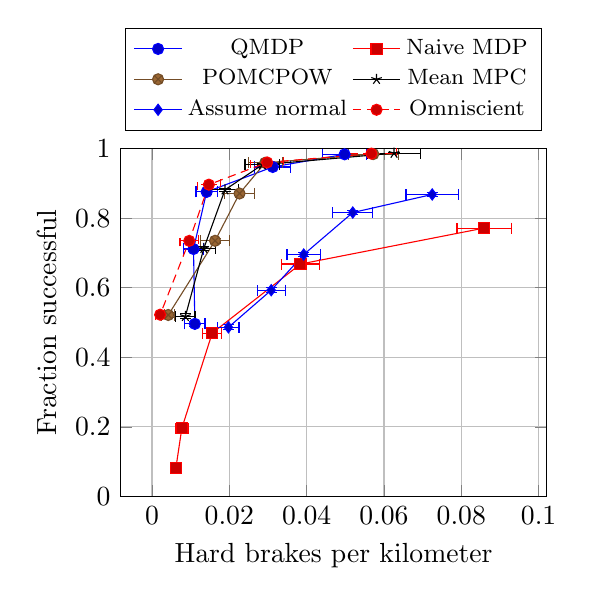
\begin{tikzpicture}[]
\begin{axis}[height = {6cm}, ylabel = {Fraction successful}, ymax = {1.0}, xlabel = {Hard brakes per kilometer}, legend style={at={(0.5,1.05)}, anchor=south, font=\footnotesize}, legend columns=2, grid=both, xticklabel style={/pgf/number format/fixed, /pgf/number format/precision=2}, ymin = {0.0}, width = {7cm}]\addplot+ [
, error bars/.cd, 
x dir=both, x explicit, y dir=both, y explicit]
table [
x error plus=ex+, x error minus=ex-, y error plus=ey+, y error minus=ey-
] {
x y ex+ ex- ey+ ey-
0.04982981000707848 0.9834 0.005706248391264743 0.005706248391264743 0.0018070808250384592 0.0018070808250384592
0.031232783596988736 0.947 0.004668205805406493 0.004668205805406493 0.0031686287320555903 0.0031686287320555903
0.014140495513949719 0.8754 0.0027387047291886337 0.0027387047291886337 0.004671116768651089 0.004671116768651089
0.010740007530656943 0.7112 0.0025248322247608855 0.0025248322247608855 0.006409924291743685 0.006409924291743685
0.01109744050066768 0.496 0.0026314249494763134 0.0026314249494763134 0.0070715487243087185 0.0070715487243087185
};
\addlegendentry{QMDP}
\addplot+ [
, error bars/.cd, 
x dir=both, x explicit, y dir=both, y explicit]
table [
x error plus=ex+, x error minus=ex-, y error plus=ey+, y error minus=ey-
] {
x y ex+ ex- ey+ ey-
0.08592815286543948 0.7714 0.0070257612602544935 0.0070257612602544935 0.005939315035643325 0.005939315035643325
0.03840643277900424 0.668 0.00486665445597094 0.00486665445597094 0.006660636066815469 0.006660636066815469
0.015581010628548301 0.4696 0.00246857020717764 0.00246857020717764 0.007058692019532005 0.007058692019532005
0.007725156902563876 0.196 0.0015844950508215265 0.0015844950508215265 0.005614544026091883 0.005614544026091883
0.006186411204866511 0.0818 0.0013441969855230165 0.0013441969855230165 0.003876178137210714 0.003876178137210714
};
\addlegendentry{Naive MDP}
\addplot+ [
, error bars/.cd, 
x dir=both, x explicit, y dir=both, y explicit]
table [
x error plus=ex+, x error minus=ex-, y error plus=ey+, y error minus=ey-
] {
x y ex+ ex- ey+ ey-
0.057250781704335126 0.984 0.006528764780903003 0.006528764780903003 0.0017746633162313392 0.0017746633162313392
0.02927402353166062 0.959 0.004381808918702063 0.004381808918702063 0.002804527246188737 0.002804527246188737
0.02264634746138381 0.8708 0.0038952692679507356 0.0038952692679507356 0.0047440460784692095 0.0047440460784692095
0.016312281093638848 0.7348 0.0037838063718228605 0.0037838063718228605 0.006243523710026526 0.006243523710026526
0.004209628232537873 0.5216 0.0016879515277842213 0.0016879515277842213 0.007065173128400112 0.007065173128400112
};
\addlegendentry{POMCPOW}
\addplot+ [
, error bars/.cd, 
x dir=both, x explicit, y dir=both, y explicit]
table [
x error plus=ex+, x error minus=ex-, y error plus=ey+, y error minus=ey-
] {
x y ex+ ex- ey+ ey-
0.06260483925695728 0.9866 0.006835162140577933 0.006835162140577933 0.0016262278202591003 0.0016262278202591003
0.02854114963264953 0.9534 0.004472363049810522 0.004472363049810522 0.0029811852497117165 0.0029811852497117165
0.018891089897816835 0.8814 0.003499161204501022 0.003499161204501022 0.004572853616511231 0.004572853616511231
0.013411593483221355 0.7132 0.003059405212297941 0.003059405212297941 0.006396665964945574 0.006396665964945574
0.008640121551458229 0.5176 0.002494154850621593 0.002494154850621593 0.0070673925607342486 0.0070673925607342486
};
\addlegendentry{Mean MPC}
\addplot+ [
, error bars/.cd, 
x dir=both, x explicit, y dir=both, y explicit]
table [
x error plus=ex+, x error minus=ex-, y error plus=ey+, y error minus=ey-
] {
x y ex+ ex- ey+ ey-
0.07248586845463478 0.868 0.00677120845795259 0.00677120845795259 0.004787461118044853 0.004787461118044853
0.05193311339416217 0.816 0.005151792492112015 0.005151792492112015 0.0054804020802667695 0.0054804020802667695
0.03924644806450444 0.6954 0.004313148197834641 0.004313148197834641 0.006509396473444352 0.006509396473444352
0.030837184686467223 0.5928 0.0036046152283785594 0.0036046152283785594 0.006948905630233565 0.006948905630233565
0.019772105226155662 0.4862 0.0027424439024956275 0.0027424439024956275 0.007069081013913758 0.007069081013913758
};
\addlegendentry{Assume normal}
\addplot+ [
, error bars/.cd, 
x dir=both, x explicit, y dir=both, y explicit]
table [
x error plus=ex+, x error minus=ex-, y error plus=ey+, y error minus=ey-
] {
x y ex+ ex- ey+ ey-
0.05675463383042475 0.9854 0.006381874200695258 0.006381874200695258 0.0016964502906710076 0.0016964502906710076
0.029783665217331123 0.96 0.004328833952023721 0.004328833952023721 0.002771558461815559 0.002771558461815559
0.014713087880870836 0.8962 0.0029827123860535604 0.0029827123860535604 0.004313795749308628 0.004313795749308628
0.009642380002978125 0.7346 0.0023853674802869727 0.0023853674802869727 0.006245027467803034 0.006245027467803034
0.0021140562847594543 0.5224 0.0011203034712754722 0.0011203034712754722 0.007064674792655703 0.007064674792655703
};
\addlegendentry{Omniscient}
\end{axis}

\end{tikzpicture}

        \end{center}
        \caption{Fully correlated ($\rho=1$)}
    \end{subfigure}
    \hfill
    \begin{subfigure}[b]{0.48\textwidth}
        \begin{center}
            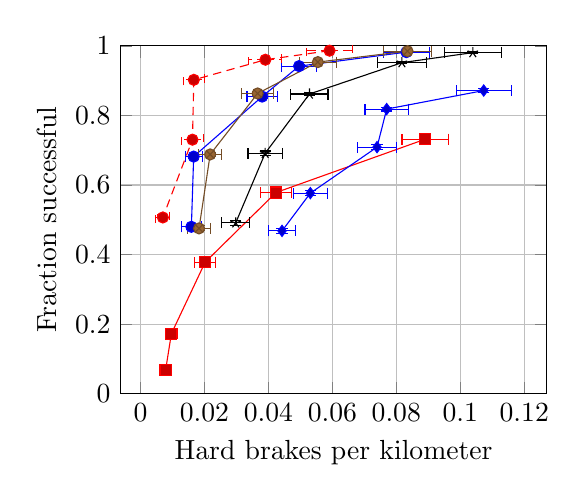
\begin{tikzpicture}[]
\begin{axis}[height = {6cm}, ylabel = {Fraction successful}, ymax = {1.0}, xlabel = {Hard brakes per kilometer}, legend style={at={(0.5,1.05)}, anchor=south, font=\footnotesize}, legend columns=2, grid=both, xticklabel style={/pgf/number format/fixed, /pgf/number format/precision=2}, ymin = {0.0}, width = {7cm}]\addplot+ [
, error bars/.cd, 
x dir=both, x explicit, y dir=both, y explicit]
table [
x error plus=ex+, x error minus=ex-, y error plus=ey+, y error minus=ey-
] {
x y ex+ ex- ey+ ey-
0.0831451030883629 0.9818 0.007114079655369576 0.007114079655369576 0.0018906260585791856 0.0018906260585791856
0.049588695018966185 0.9416 0.005495017124049245 0.005495017124049245 0.0033166380594818385 0.0033166380594818385
0.038041083261445195 0.854 0.004727003229891565 0.004727003229891565 0.004994175443220966 0.004994175443220966
0.016638561050694296 0.6816 0.002693404962471551 0.002693404962471551 0.006588851993641919 0.006588851993641919
0.015922997816150336 0.4798 0.0030510754966022453 0.0030510754966022453 0.007066001533790888 0.007066001533790888
};
\addplot+ [
, error bars/.cd, 
x dir=both, x explicit, y dir=both, y explicit]
table [
x error plus=ex+, x error minus=ex-, y error plus=ey+, y error minus=ey-
] {
x y ex+ ex- ey+ ey-
0.08898230662559689 0.7314 0.007199203137779685 0.007199203137779685 0.006268864947783357 0.006268864947783357
0.0423851053519722 0.5782 0.0048715579593175936 0.0048715579593175936 0.006984748337761956 0.006984748337761956
0.02022593684885273 0.378 0.003194299329247237 0.003194299329247237 0.006858032263069643 0.006858032263069643
0.009668571203540983 0.1726 0.0017731878923584546 0.0017731878923584546 0.005344863095749249 0.005344863095749249
0.007852578628305816 0.0672 0.0014959428905968657 0.0014959428905968657 0.0035410930329452914 0.0035410930329452914
};
\addplot+ [
, error bars/.cd, 
x dir=both, x explicit, y dir=both, y explicit]
table [
x error plus=ex+, x error minus=ex-, y error plus=ey+, y error minus=ey-
] {
x y ex+ ex- ey+ ey-
0.08350450937311038 0.9846 0.007510710816478812 0.007510710816478812 0.001741601169879885 0.001741601169879885
0.05546440644100046 0.9532 0.005803935970743728 0.005803935970743728 0.0029872624168876577 0.0029872624168876577
0.03663720575250644 0.863 0.005072294801460488 0.005072294801460488 0.0048632222020011835 0.0048632222020011835
0.02179862080641367 0.6878 0.003573426729756362 0.003573426729756362 0.006553992902391117 0.006553992902391117
0.01831218661199491 0.4752 0.0037142551685492467 0.0037142551685492467 0.0070630708189765926 0.0070630708189765926
};
\addplot+ [
, error bars/.cd, 
x dir=both, x explicit, y dir=both, y explicit]
table [
x error plus=ex+, x error minus=ex-, y error plus=ey+, y error minus=ey-
] {
x y ex+ ex- ey+ ey-
0.10391648370554485 0.9804 0.008874239757182123 0.008874239757182123 0.0019605960285988197 0.0019605960285988197
0.08175580010229523 0.9516 0.007724653344890724 0.007724653344890724 0.003035346877398558 0.003035346877398558
0.05283994220509099 0.8614 0.005809829961129406 0.005809829961129406 0.004887001591662435 0.004887001591662435
0.03898666963114873 0.691 0.005368692950549745 0.005368692950549745 0.006535468037447208 0.006535468037447208
0.029779406469016625 0.491 0.004362096969349006 0.004362096969349006 0.00707062930436548 0.00707062930436548
};
\addplot+ [
, error bars/.cd, 
x dir=both, x explicit, y dir=both, y explicit]
table [
x error plus=ex+, x error minus=ex-, y error plus=ey+, y error minus=ey-
] {
x y ex+ ex- ey+ ey-
0.1073320377110703 0.8714 0.008637398563332814 0.008637398563332814 0.004734647967724278 0.004734647967724278
0.07699317128339683 0.8182 0.00679509030021899 0.00679509030021899 0.005454878838308729 0.005454878838308729
0.07396993712098031 0.7088 0.00610758714324605 0.00610758714324605 0.00642563380173123 0.00642563380173123
0.0531187846661916 0.5766 0.005255076500404298 0.005255076500404298 0.0069882941588809795 0.0069882941588809795
0.04426741706462751 0.468 0.00432639641808174 0.00432639641808174 0.007057277168441554 0.007057277168441554
};
\addplot+ [
, error bars/.cd, 
x dir=both, x explicit, y dir=both, y explicit]
table [
x error plus=ex+, x error minus=ex-, y error plus=ey+, y error minus=ey-
] {
x y ex+ ex- ey+ ey-
0.05911726368909217 0.986 0.007133118891728767 0.007133118891728767 0.0016617317083254147 0.0016617317083254147
0.03906509256487092 0.96 0.0051688472410064265 0.0051688472410064265 0.0027715584618155584 0.0027715584618155584
0.01668998208126091 0.9022 0.0032762838268948443 0.0032762838268948443 0.004201257206173249 0.004201257206173249
0.016254632652627846 0.7302 0.0033975262242862186 0.0033975262242862186 0.006277696543699677 0.006277696543699677
0.007004856650780219 0.5066 0.002204575783184311 0.002204575783184311 0.007071158904850855 0.007071158904850855
};
\end{axis}

\end{tikzpicture}

        \end{center}
        \caption{Partially correlated ($\rho=0.75$)}
    \end{subfigure}
    
    \centering
    \caption{Average hard braking frequency and success rate}
    \label{fig:bpkm}
\end{figure}


\subsubsection{Correlation comparison}

It is also interesting to consider the Affect that the correlation between model parameters has on the relative effectiveness of the control approaches.
\Cref{fig:000} shows that when there is no correlation, QMDP offers a significant advantage over mean MPC, and POMCPOW offers a further significant advantage over QMDP.
In this case, since the parameters are uncorrelated, there is a large amount of uncertainty in them even when some (e.g. $\dot{x}_0$) are easy to observe, and since POMCPOW is able to plan into the future considering this uncertainty, it performs better.
On the other hand, when the parameters are fully correlated as shown in \cref{fig:100}, all of the parameters are easy to estimate by observing only a few, so there is not a significant performance gap between mean MPC, QMDP, and POMCPOW; all are able to close the gap and achieve nearly the same performance as the upper bound.
\Cref{fig:075} shows the expected behavior between the extremes.

\Cref{fig:corplot} shows the performance gaps at more points between $\rho=0$ and $1$.
As the correlation increases, the approximate POMDP planning approaches get steadily closer to closing the performance gap with the upper bound.
These results have significant implications for the real world.
It suggests that if most human driver behavior is correlated with easily measurable quantities, near-optimal performance can be achieved by simpler approaches like mean MPC.
If there is little correlation, planning with internal states offers a less pronounced benefit, and more advanced planners that carry the uncertainty further into the future are needed to realize that benefit.

\begin{figure}[htbp]
    \centering
    % \includestandalone[mode=buildnew,width=0.5\textwidth]{media/corplot}
    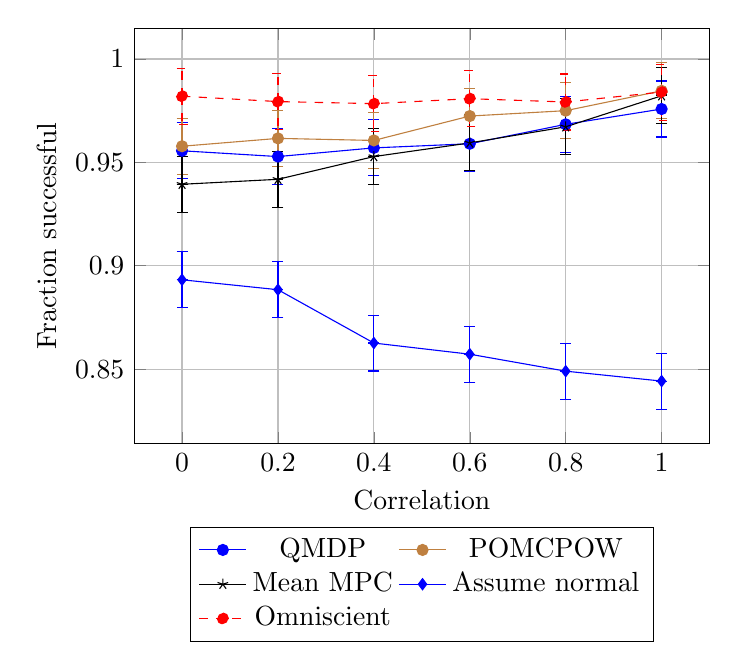
\begin{tikzpicture}[]
\begin{axis}[height = {2.7in}, ylabel = {Fraction successful}, xlabel = {Correlation}, legend style={at={(0.5,-0.2)}, anchor=north}, legend columns=2, grid=both, width = {3.5in}]\addplot+ [
mark = {*}, blue, mark options={fill=blue}, error bars/.cd, 
x dir=both, x explicit, y dir=both, y explicit]
table [
x error plus=ex+, x error minus=ex-, y error plus=ey+, y error minus=ey-
] {
x y ex+ ex- ey+ ey-
0.0 0.9556 0.0 0.0 0.01353728726055671 0.01353728726055671
0.2 0.9528 0.0 0.0 0.01353728726055671 0.01353728726055671
0.4 0.957 0.0 0.0 0.01353728726055671 0.01353728726055671
0.6 0.959 0.0 0.0 0.01353728726055671 0.01353728726055671
0.8 0.9684 0.0 0.0 0.01353728726055671 0.01353728726055671
1.0 0.9758 0.0 0.0 0.01353728726055671 0.01353728726055671
};
\addlegendentry{QMDP}
\addplot+ [
mark = {*}, brown, mark options={fill=brown}, error bars/.cd, 
x dir=both, x explicit, y dir=both, y explicit]
table [
x error plus=ex+, x error minus=ex-, y error plus=ey+, y error minus=ey-
] {
x y ex+ ex- ey+ ey-
0.0 0.9578 0.0 0.0 0.01353728726055671 0.01353728726055671
0.2 0.9616 0.0 0.0 0.01353728726055671 0.01353728726055671
0.4 0.9606 0.0 0.0 0.01353728726055671 0.01353728726055671
0.6 0.9724 0.0 0.0 0.01353728726055671 0.01353728726055671
0.8 0.975 0.0 0.0 0.01353728726055671 0.01353728726055671
1.0 0.9846 0.0 0.0 0.01353728726055671 0.01353728726055671
};
\addlegendentry{POMCPOW}
\addplot+ [
mark = {star}, black, mark options={fill=black}, error bars/.cd, 
x dir=both, x explicit, y dir=both, y explicit]
table [
x error plus=ex+, x error minus=ex-, y error plus=ey+, y error minus=ey-
] {
x y ex+ ex- ey+ ey-
0.0 0.9394 0.0 0.0 0.01353728726055671 0.01353728726055671
0.2 0.9418 0.0 0.0 0.01353728726055671 0.01353728726055671
0.4 0.9528 0.0 0.0 0.01353728726055671 0.01353728726055671
0.6 0.9594 0.0 0.0 0.01353728726055671 0.01353728726055671
0.8 0.9672 0.0 0.0 0.01353728726055671 0.01353728726055671
1.0 0.9822 0.0 0.0 0.01353728726055671 0.01353728726055671
};
\addlegendentry{Mean MPC}
\addplot+ [
mark = {diamond*}, blue, mark options={fill=blue}, error bars/.cd, 
x dir=both, x explicit, y dir=both, y explicit]
table [
x error plus=ex+, x error minus=ex-, y error plus=ey+, y error minus=ey-
] {
x y ex+ ex- ey+ ey-
0.0 0.8932 0.0 0.0 0.01353728726055671 0.01353728726055671
0.2 0.8884 0.0 0.0 0.01353728726055671 0.01353728726055671
0.4 0.8626 0.0 0.0 0.01353728726055671 0.01353728726055671
0.6 0.8572 0.0 0.0 0.01353728726055671 0.01353728726055671
0.8 0.849 0.0 0.0 0.01353728726055671 0.01353728726055671
1.0 0.8442 0.0 0.0 0.01353728726055671 0.01353728726055671
};
\addlegendentry{Assume normal}
\addplot+ [
mark = {*}, red, dashed, mark options={fill=red, dashed}, error bars/.cd, 
x dir=both, x explicit, y dir=both, y explicit]
table [
x error plus=ex+, x error minus=ex-, y error plus=ey+, y error minus=ey-
] {
x y ex+ ex- ey+ ey-
0.0 0.982 0.0 0.0 0.01353728726055671 0.01353728726055671
0.2 0.9794 0.0 0.0 0.01353728726055671 0.01353728726055671
0.4 0.9784 0.0 0.0 0.01353728726055671 0.01353728726055671
0.6 0.9808 0.0 0.0 0.01353728726055671 0.01353728726055671
0.8 0.9792 0.0 0.0 0.01353728726055671 0.01353728726055671
1.0 0.984 0.0 0.0 0.01353728726055671 0.01353728726055671
};
\addlegendentry{Omniscient}
\end{axis}

\end{tikzpicture}

    \caption[Performance variation with $\Theta$ correlation]{Performance variation with $\Theta$ correlation. Success is defined as reaching the target lane within the distance limit without any unsafe actions. Error bars indicate the \SI{68}{\percent} (corresponding to one standard deviation in a normal distribution) confidence region determined by the Hoeffding Bound. The Naive MDP performance is not shown because it is significantly lower than the other approaches.}
    \label{fig:corplot}
\end{figure}

\todo{add robustness study}
